\chapter{Figures}



\section{Affinity simulation trees with stats}
\begin{figure}[!ht]
    \centering
    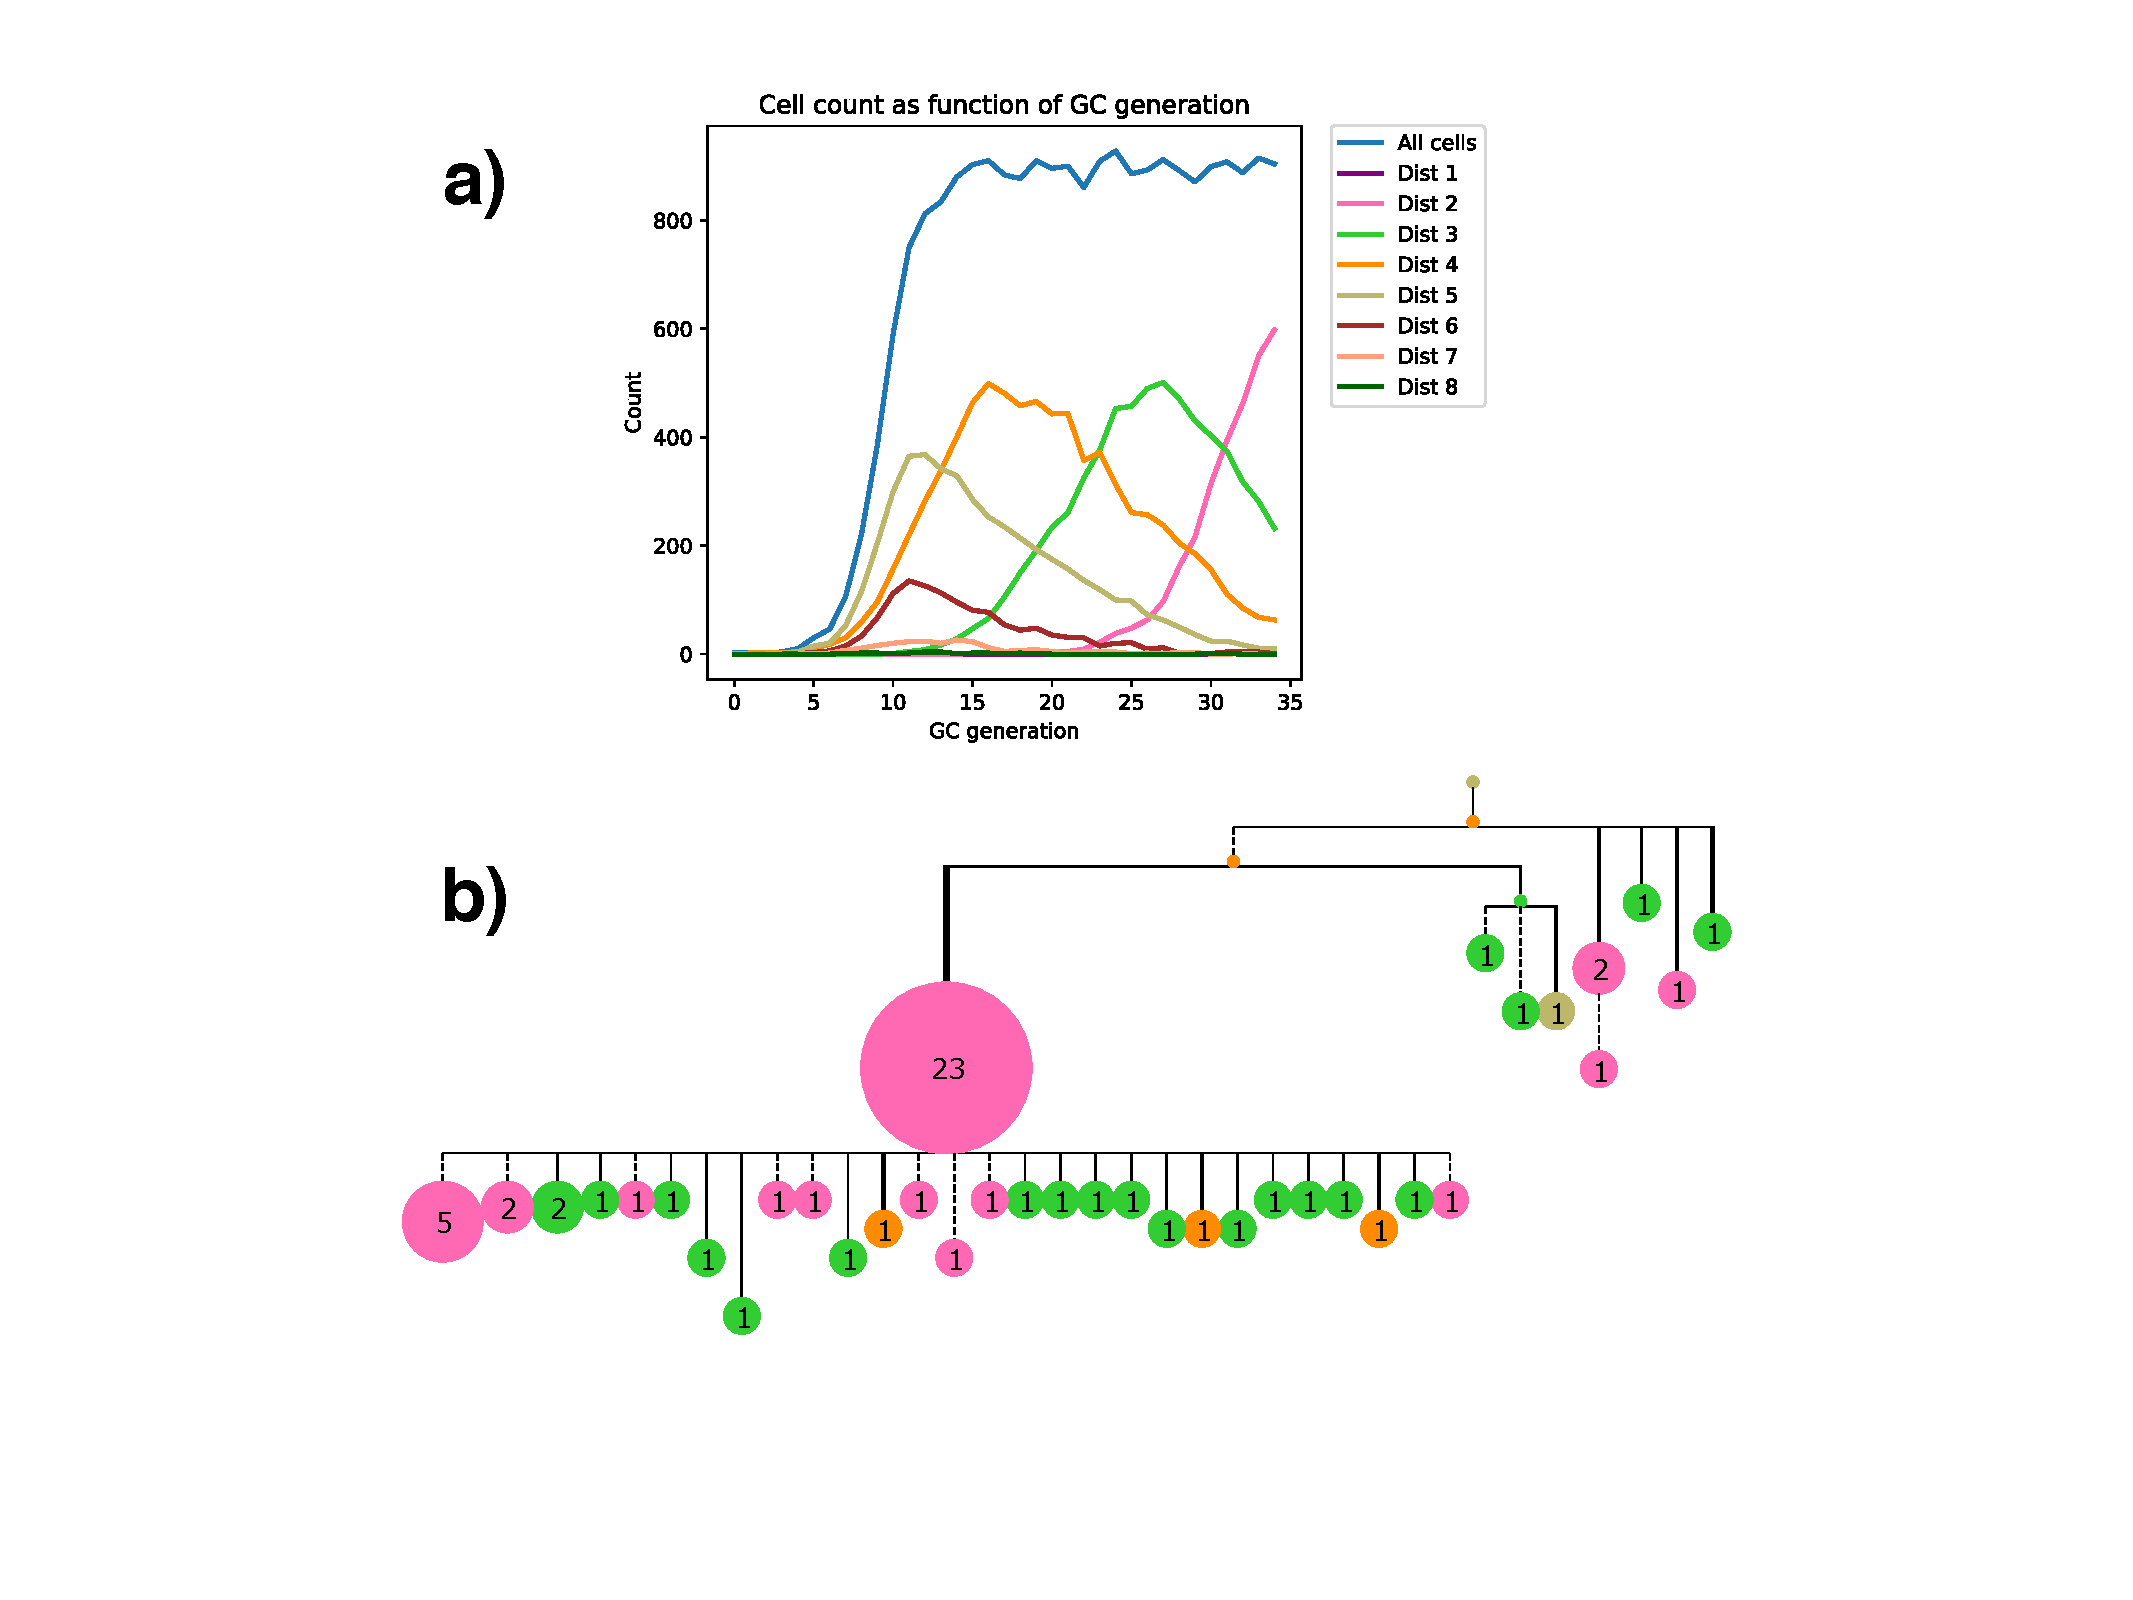
\includegraphics[width=0.8\textwidth]{figures/Tas_affsim_example_with_runstats.pdf}
    \caption{
        \label{fig:Tas_affsim_example_with_runstats}
        Summary statistics for the simulation similar to a single cell GC in figure \ref{fig:Tas_affsim_example.collapsed_runstat_color_tree}. a) run stats with color codes corresponding to affinity (through smallest distance to a target), b) resulting tree with colors matching those in a).
    }
\end{figure}





\section{Affinity simulation with visual epistasis}
\begin{figure}[!ht]
    \textbf{(a)}
    \vspace{-15mm}
    \begin{center}
    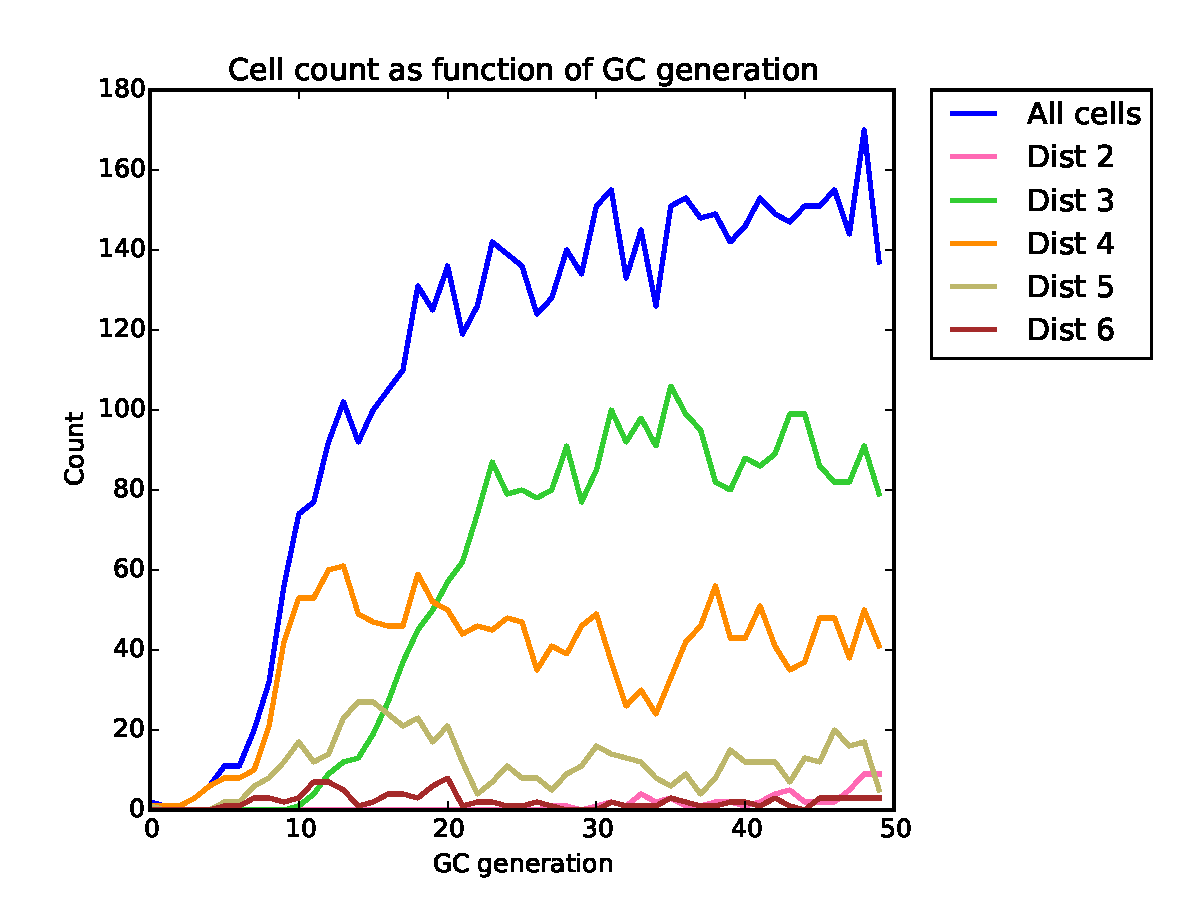
\includegraphics[width=0.6\textwidth]{figures/epi_runstats.pdf}
    \end{center}
    \textbf{(b)}
    \vspace{-15mm}
    \begin{center}
    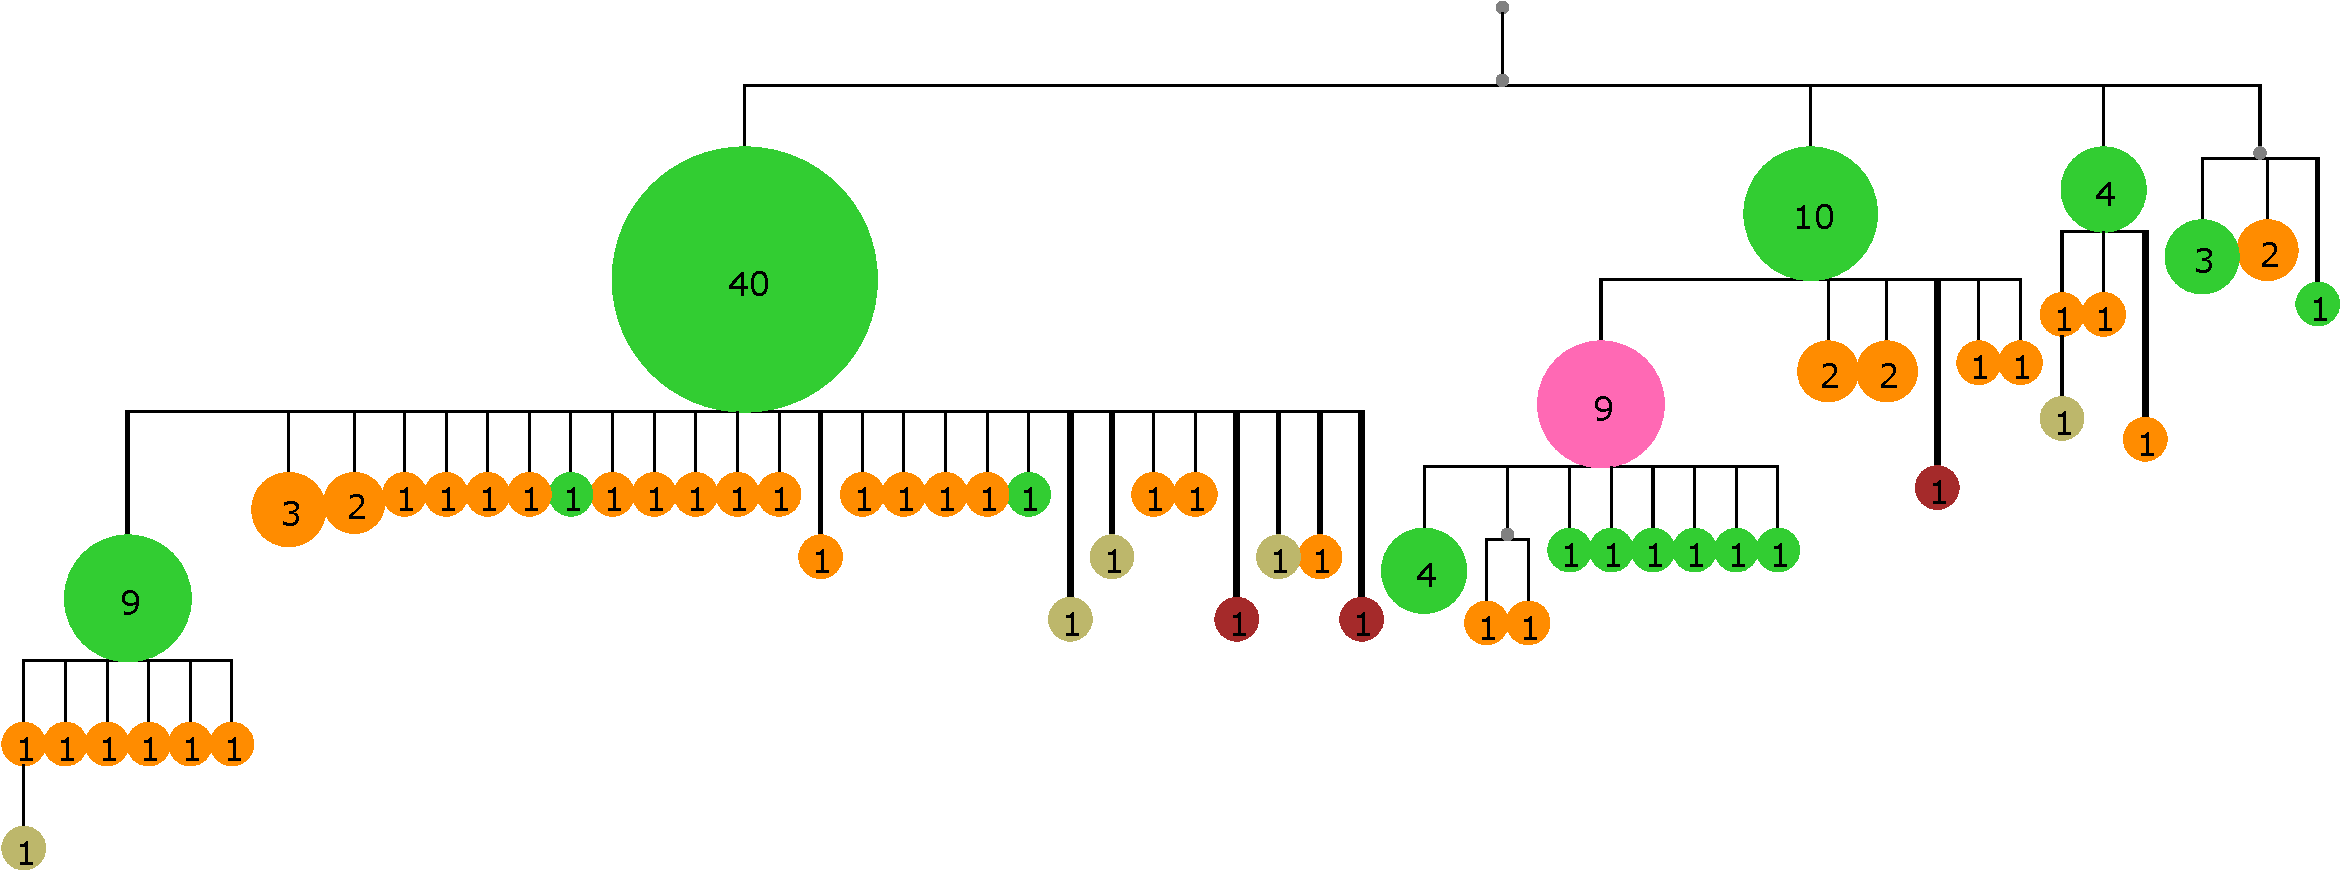
\includegraphics[width=1\textwidth]{figures/epi_collapsed_tree_runstats.pdf}
    \end{center}
    \caption{
        \label{fig:collapsed_epistasis}
        Summary statistics for the simulation showing switch in target sequences trajectories described in figure \ref{fig:epistasis_figure}. a) run stats, b) resulting tree.
        }
\end{figure}




%\iffalse


\clearpage
\section{Simulation comparison to data}
% Laura-neutsim_Laura-data
% Laura-neutsim_Tas-data   %%% Supp.

% Laura-affsim_Laura-data
% Laura-affsim_Tas-data   %%% Supp.

% Tas-neutsim_Laura-data   %%% Supp.
% Tas-neutsim_Tas-data

% Tas-affsim_Laura-data   %%% Supp.
% Tas-affsim_Tas-data

% Laura data should be referred to as HTS data
% The Tas data will be referred to as single cell data


\begin{figure}[!ht]
    \centering
    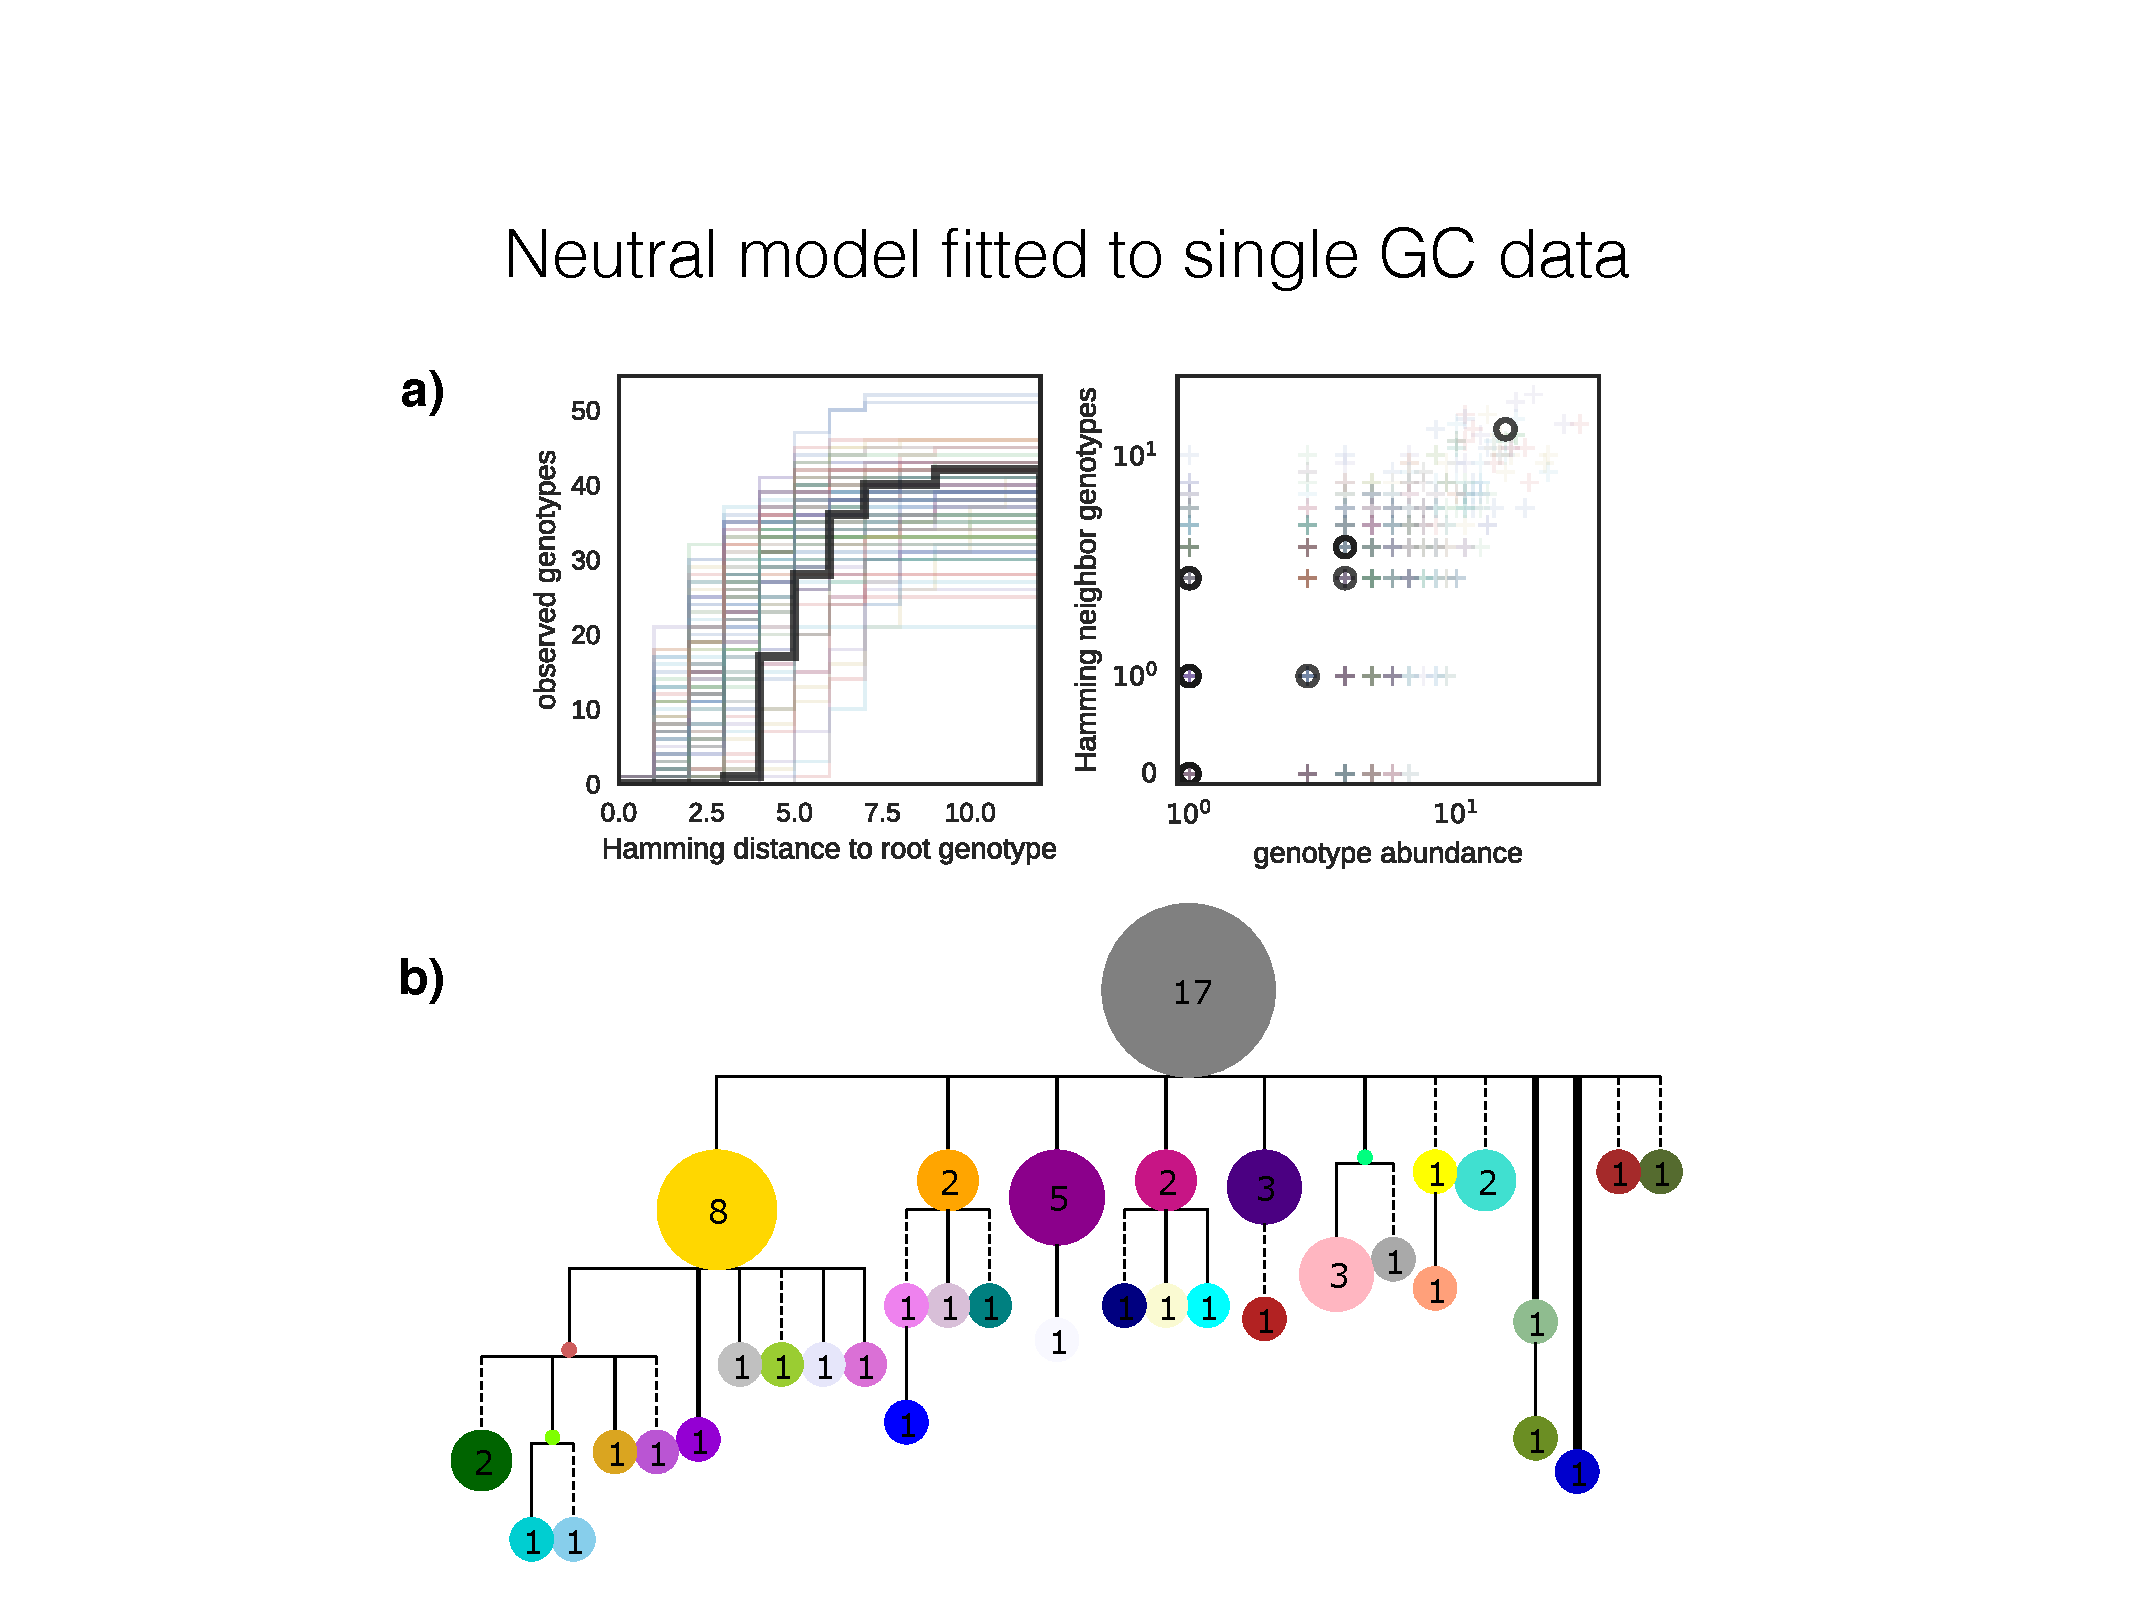
\includegraphics[width=0.8\textwidth]{figures/Tas-neutsim_runstat.pdf}
    \caption{
        \label{fig:Tas-neutsim_runstat}
        Neutral branching process with parameters fit to single cell data. In a) summary statistics of how well the simulations fit data (simulation in colors, data in black). In b) a typical tree topology from the simulation run.
    }
\end{figure}
\begin{figure}[!ht]
    \centering
    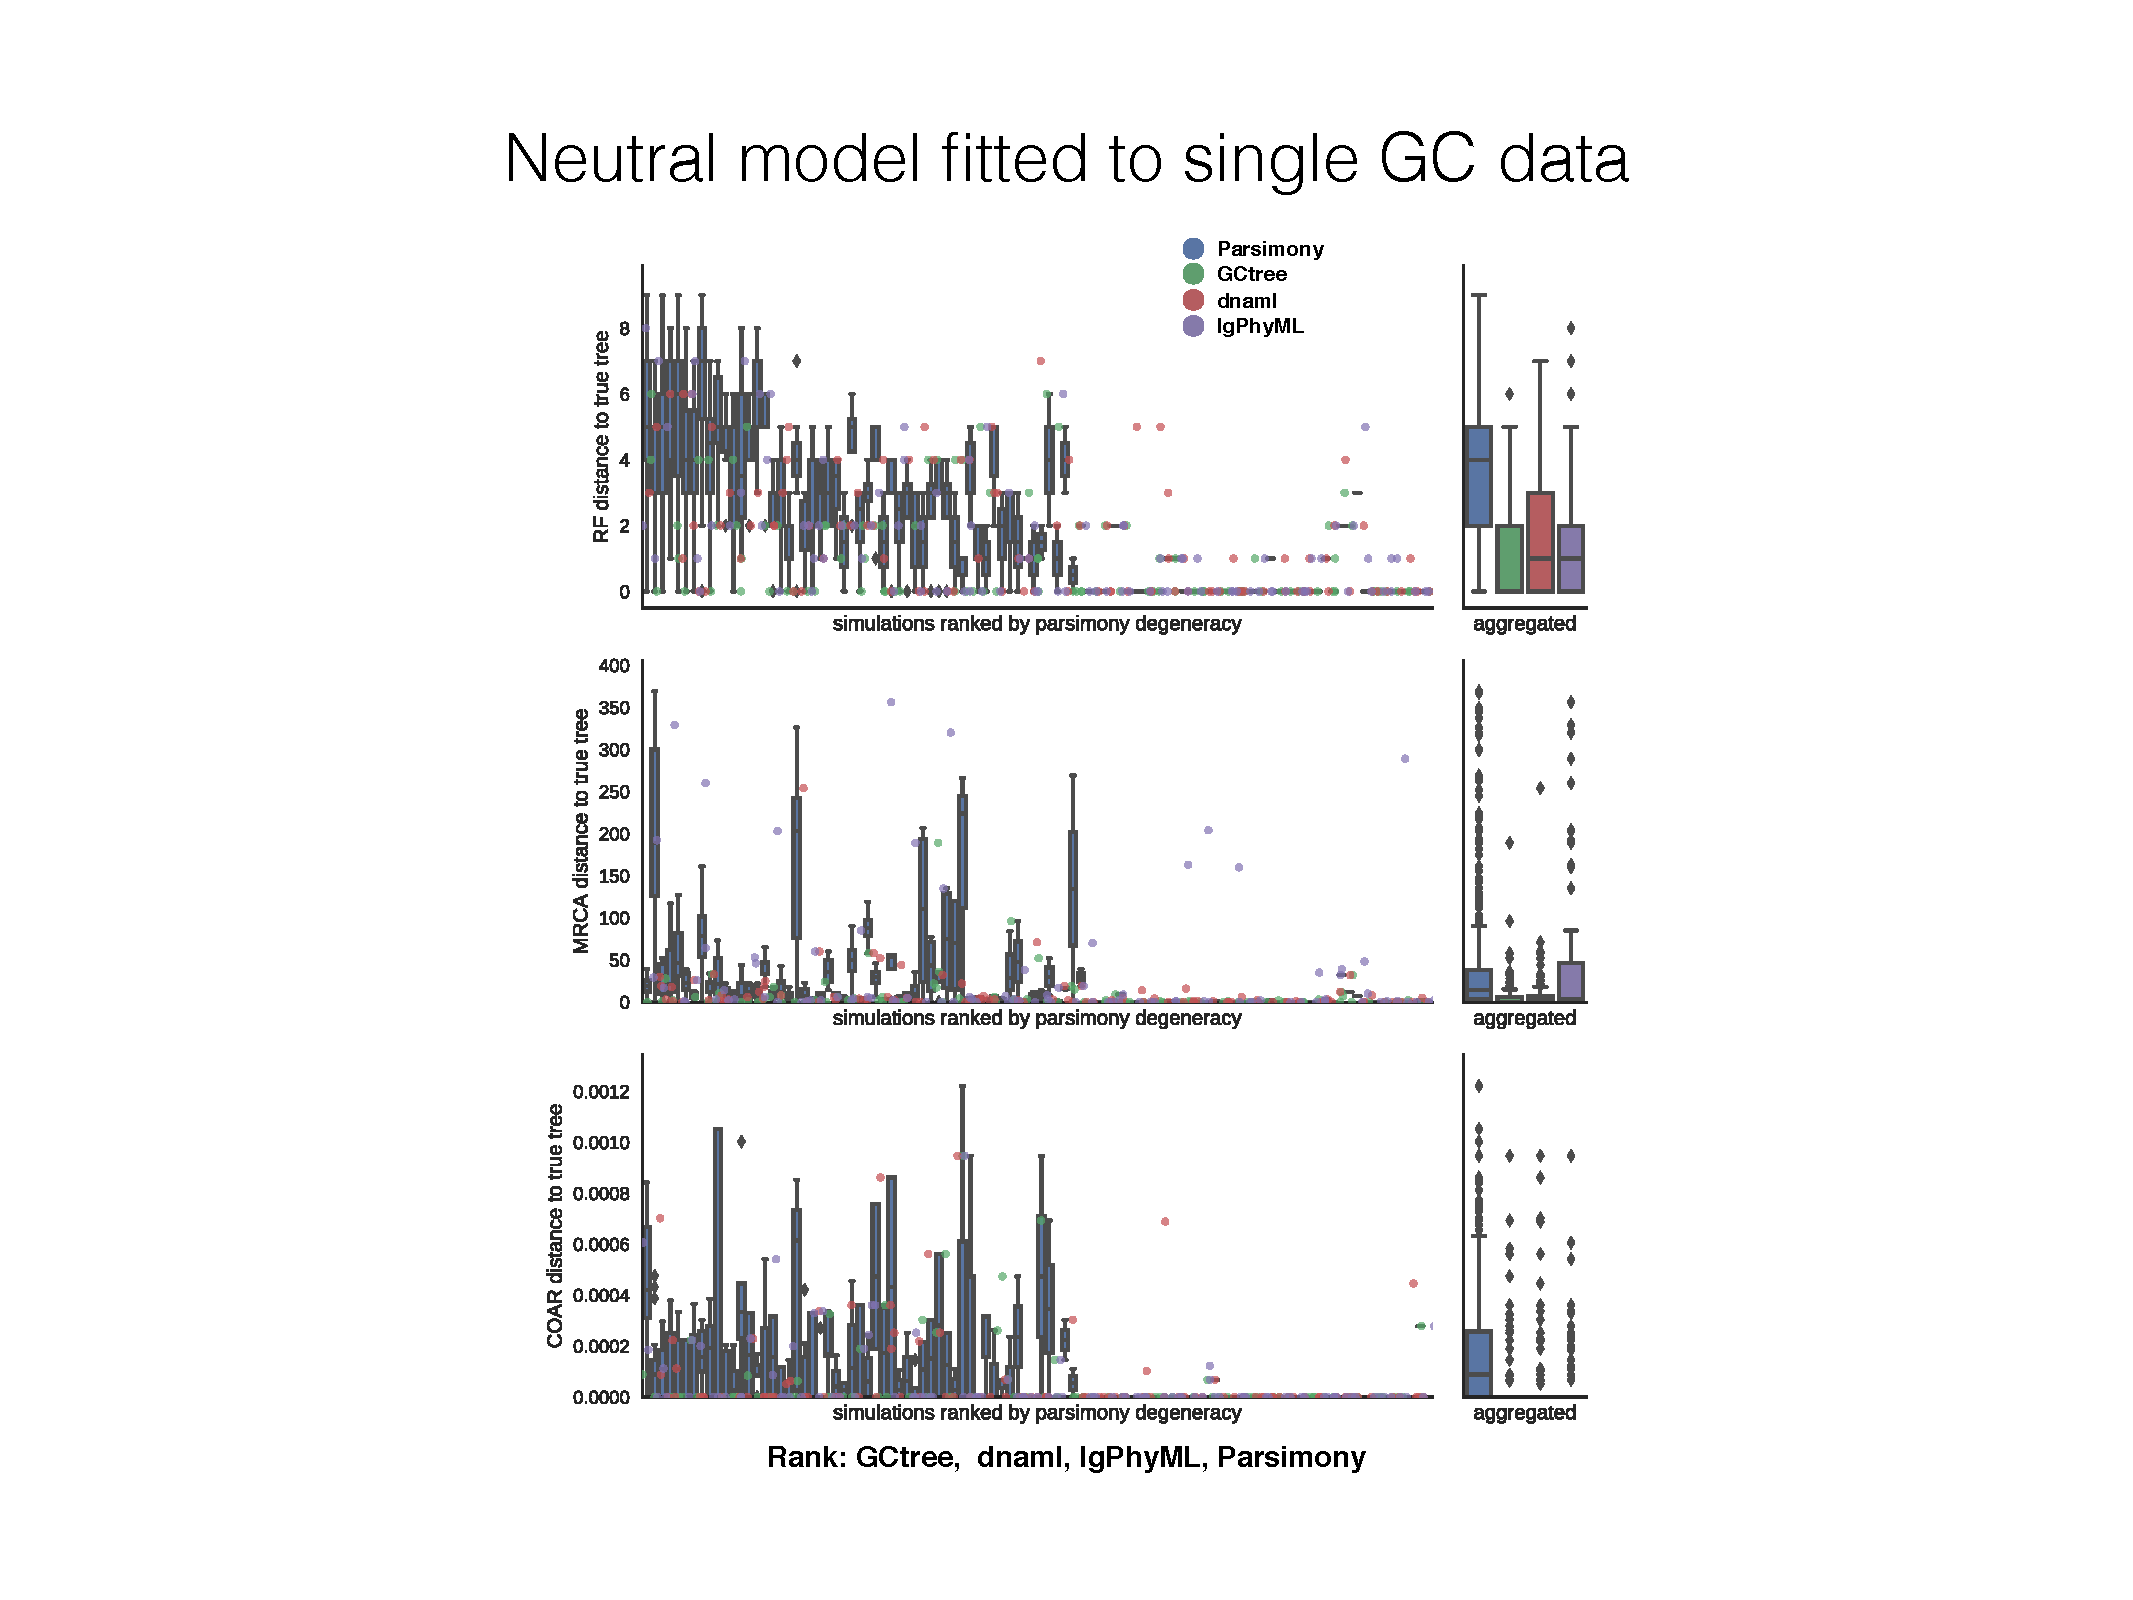
\includegraphics[width=0.8\textwidth]{figures/Tas-neutsim_vali.pdf}
    \caption{
        \label{fig:Tas-neutsim_vali}
        Performance of different inference method over the 100 simulations shown in \ref{fig:Tas-neutsim_runstat}.
        Standard box plot format with the box covering the two middle quartiles (Q2=25\% to Q3=75\% percentile), whiskers extends these and extra 1.5 times the interquartile range and points outside this are plotted individually.
        The median is indicated by a black line.
        A rank of best to worst, is subjectively decided based on the metrics plotted and with importance of the metrics determined by the rank; COAR, MRCA, RF.
    }
\end{figure}

\begin{figure}[!ht]
    \centering
    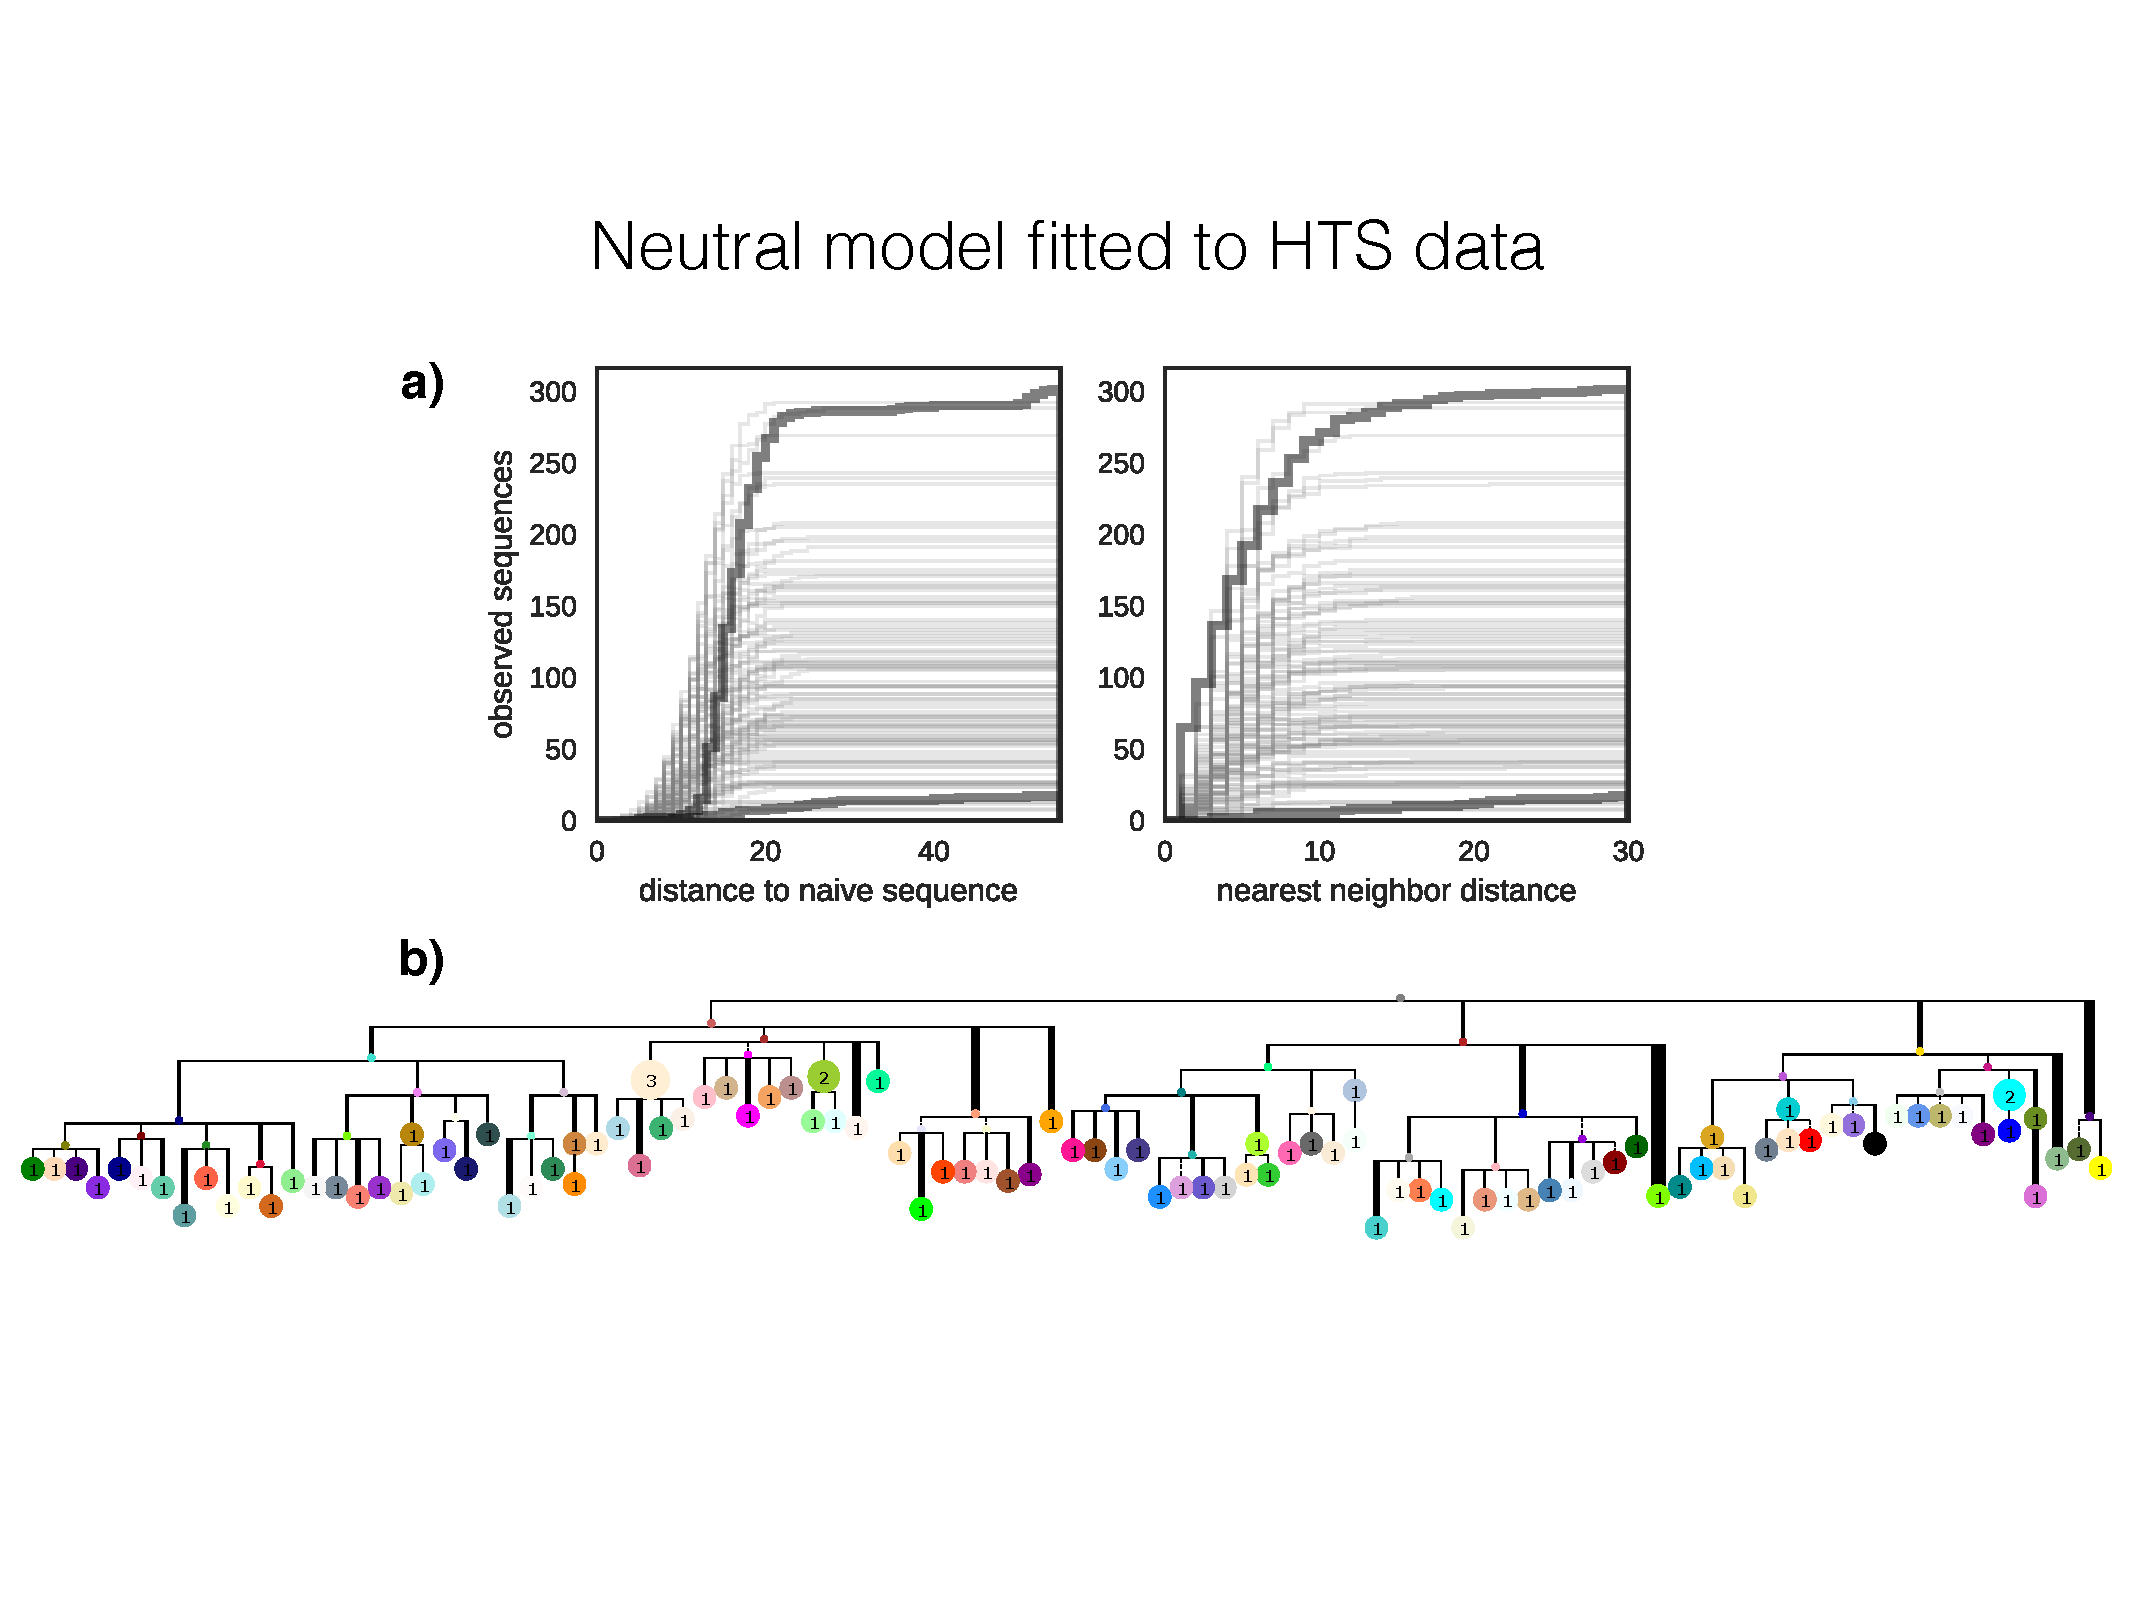
\includegraphics[width=1\textwidth]{figures/Laura-neutsim_runstat.pdf}
    \caption{
        \label{fig:Laura-neutsim_runstat}
        Neutral branching process with parameters fit to HTS data. In a) summary statistics of how well the simulations fit data (simulations in grey shade, data in dark grey). In b) a typical tree topology from the simulation run.
    }
\end{figure}
\begin{figure}
    \centering
    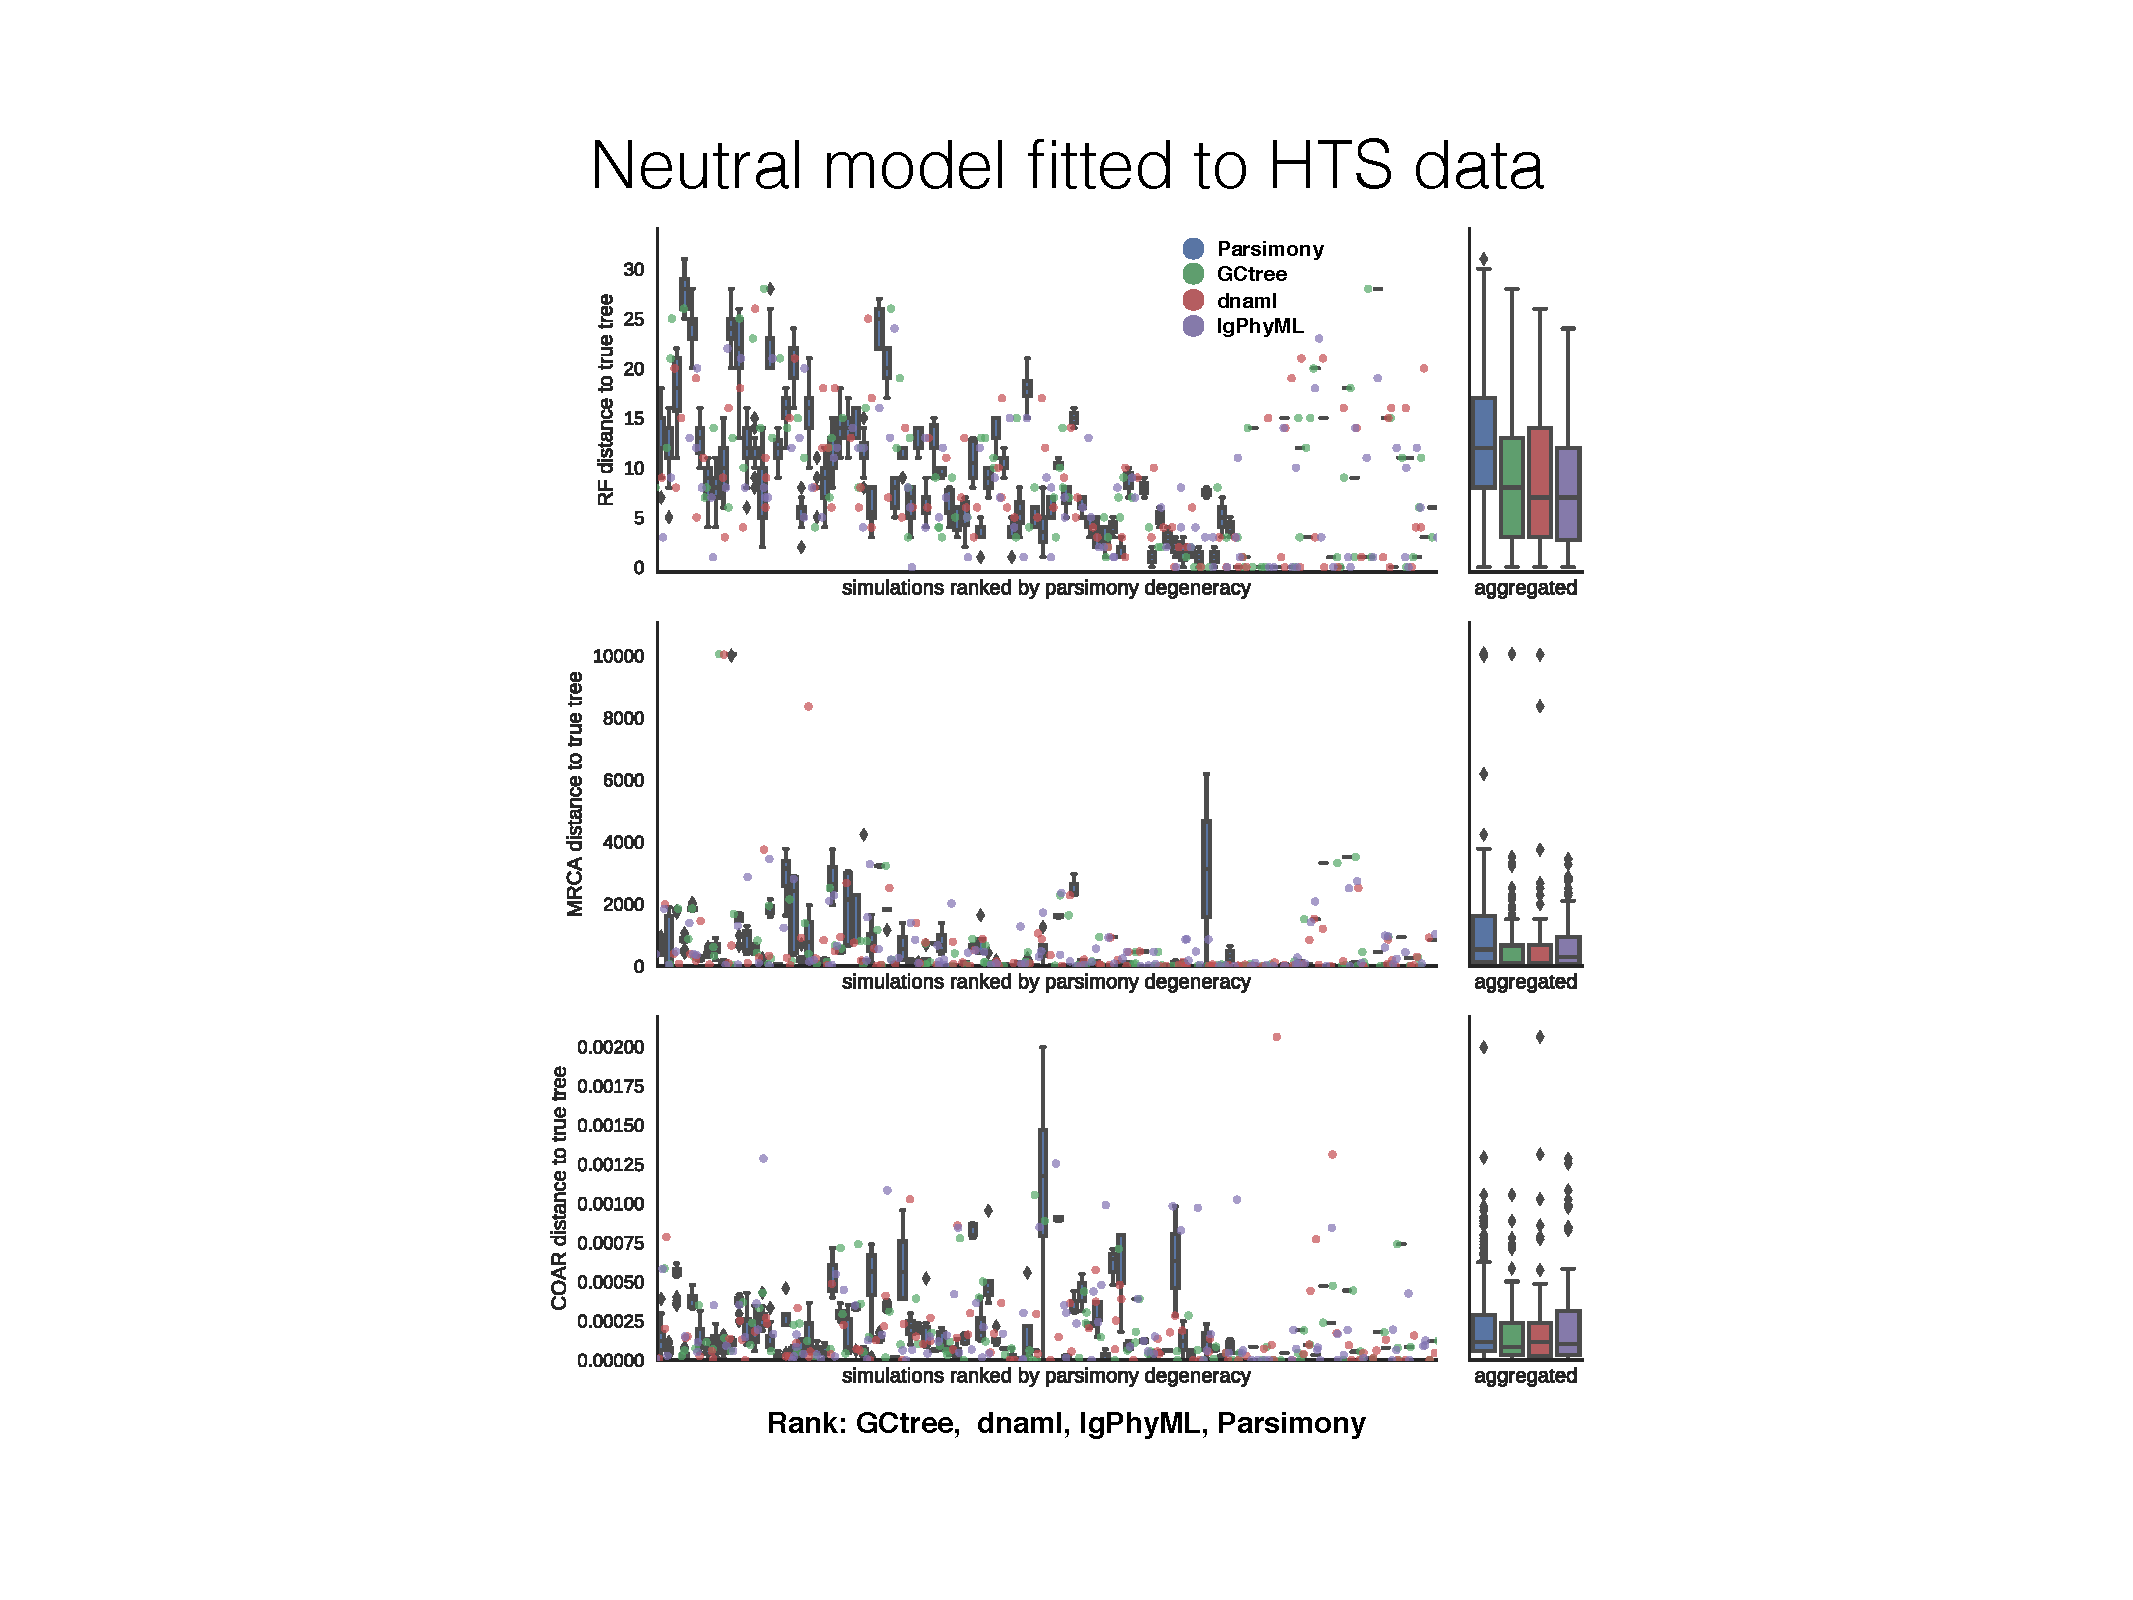
\includegraphics[width=0.8\textwidth]{figures/Laura-neutsim_vali.pdf}
    \caption{
        \label{fig:Laura-neutsim_vali}
        Performance of different inference method over the 100 simulations shown in \ref{fig:Laura-neutsim_runstat}.
        Standard box plot format with the box covering the two middle quartiles (Q2=25\% to Q3=75\% percentile), whiskers extends these and extra 1.5 times the interquartile range and points outside this are plotted individually.
        The median is indicated by a black line.
        A rank of best to worst, is subjectively decided based on the metrics plotted and with importance of the metrics determined by the rank; COAR, MRCA.
    }
\end{figure}




\begin{figure}[!ht]
    \centering
    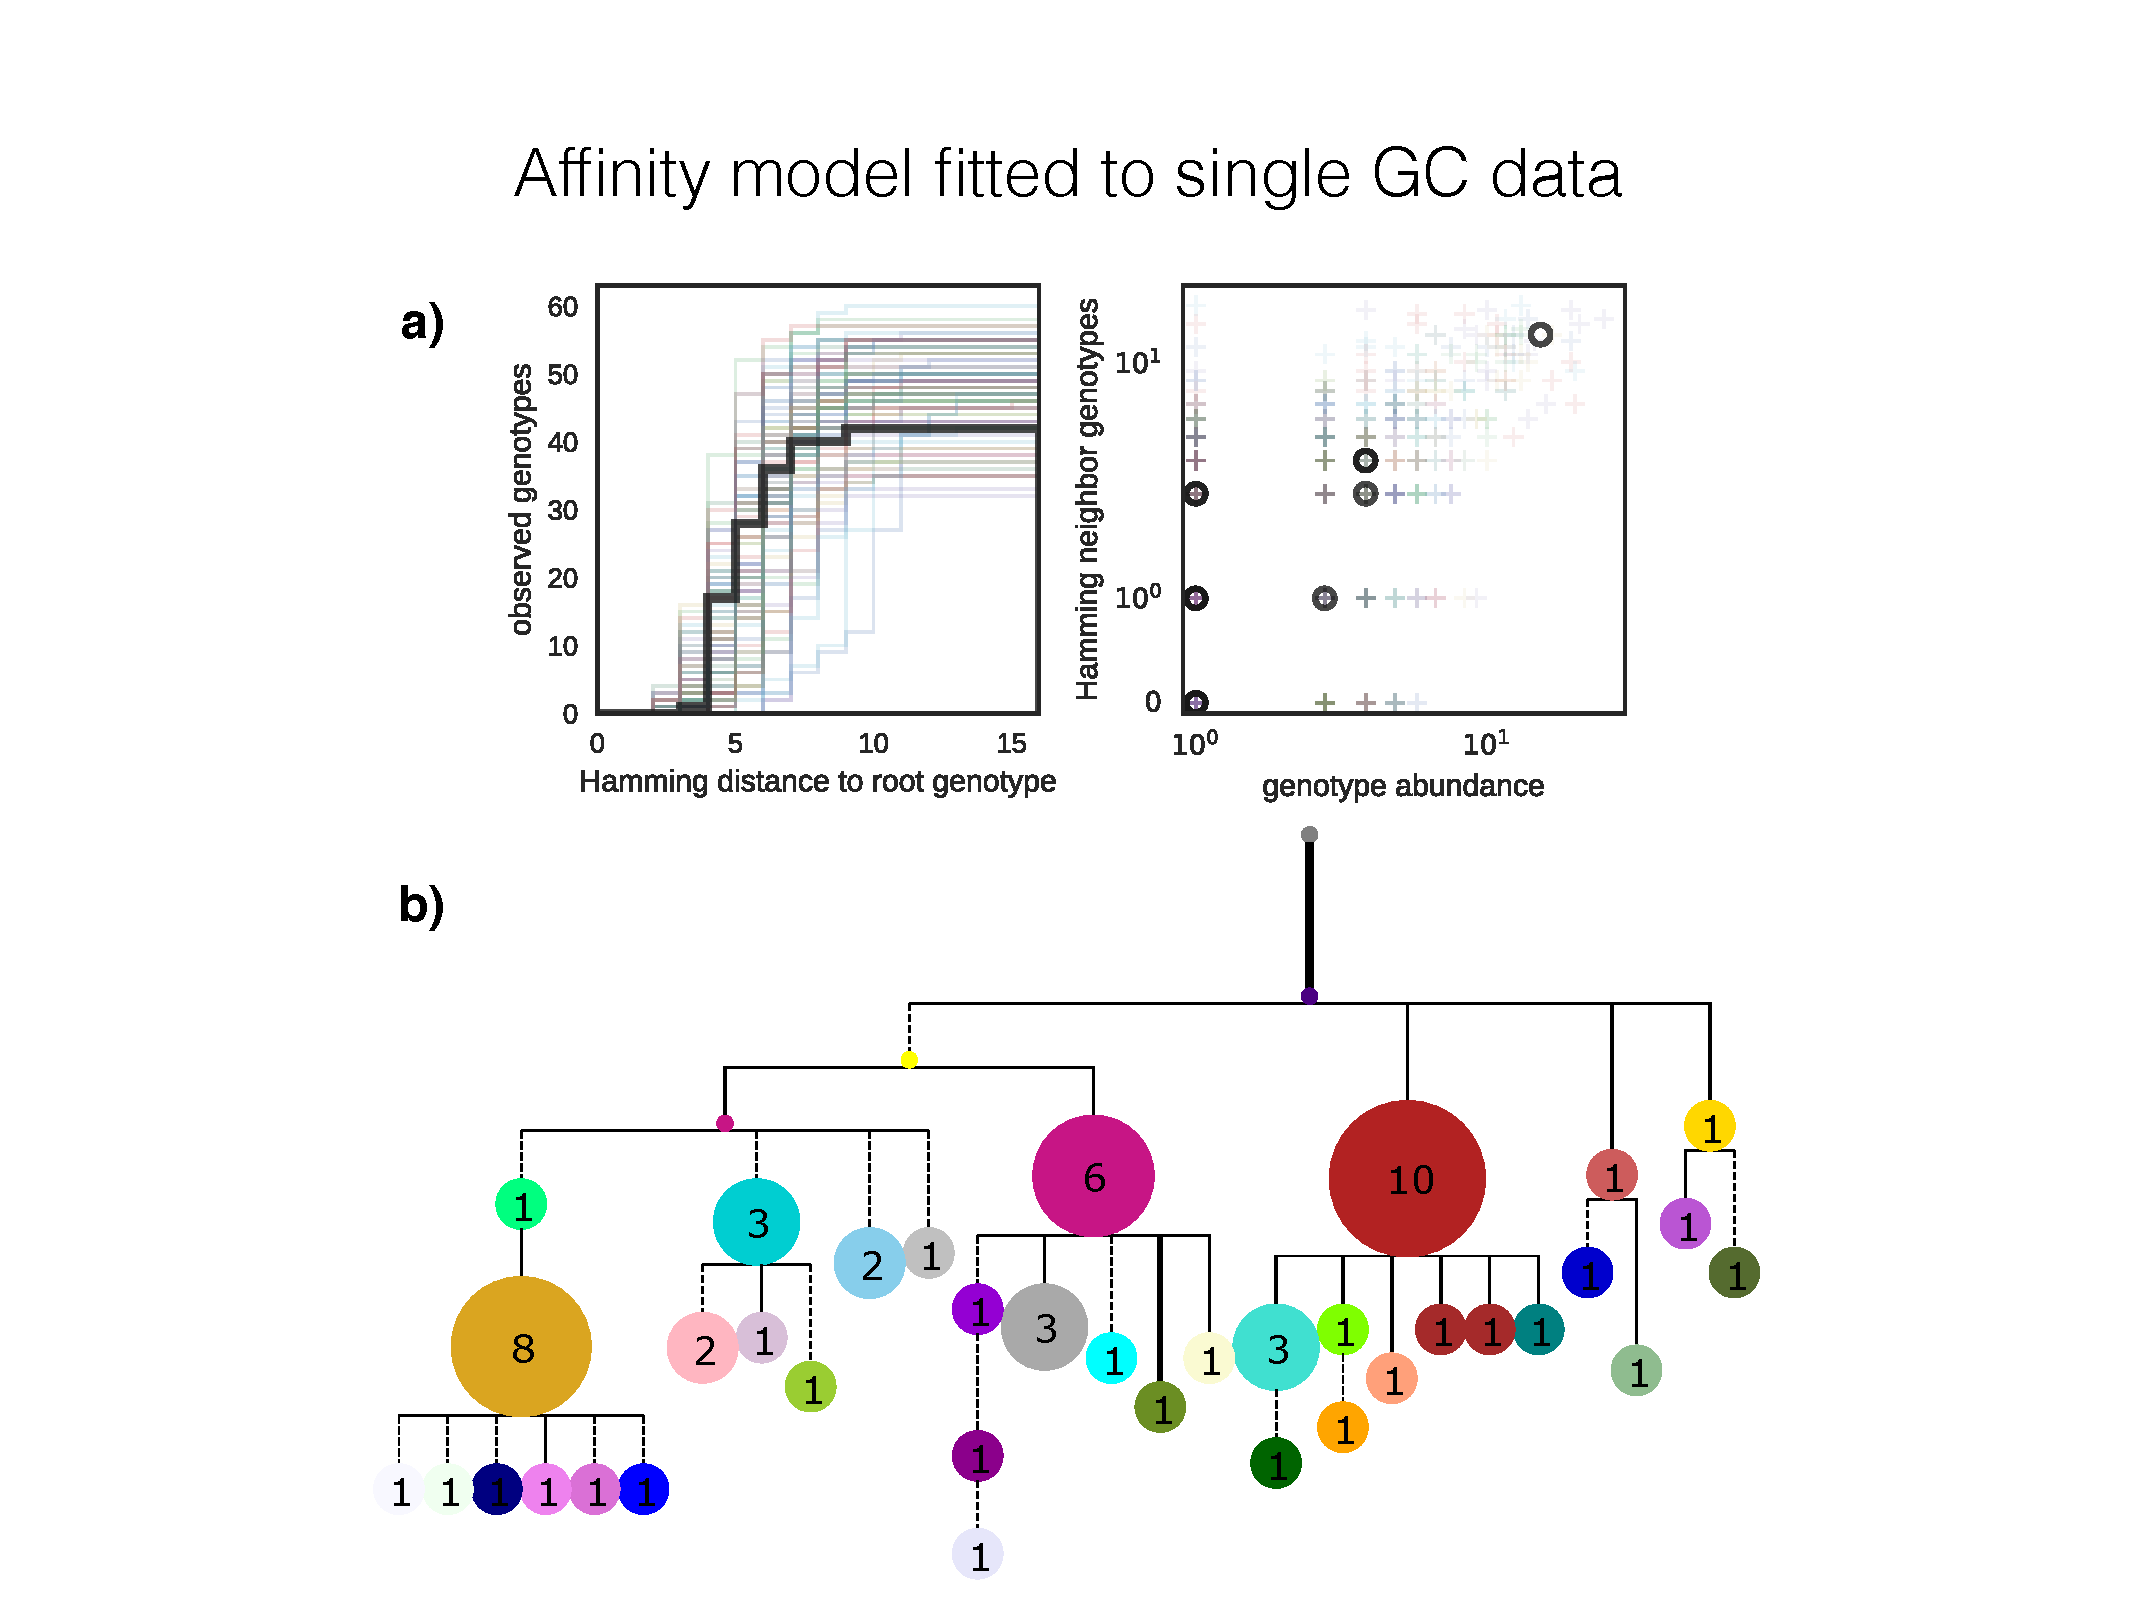
\includegraphics[width=0.8\textwidth]{figures/Tas-affsim_runstat.pdf}
    \caption{
        \label{fig:Tas-affsim_runstat}
        Affinity simulation with parameters fit to single cell data. In a) summary statistics of how well the simulations fit data (simulation in colors, data in black). In b) a typical tree topology from the simulation run.
    }
\end{figure}
\begin{figure}[!ht]
    \centering
    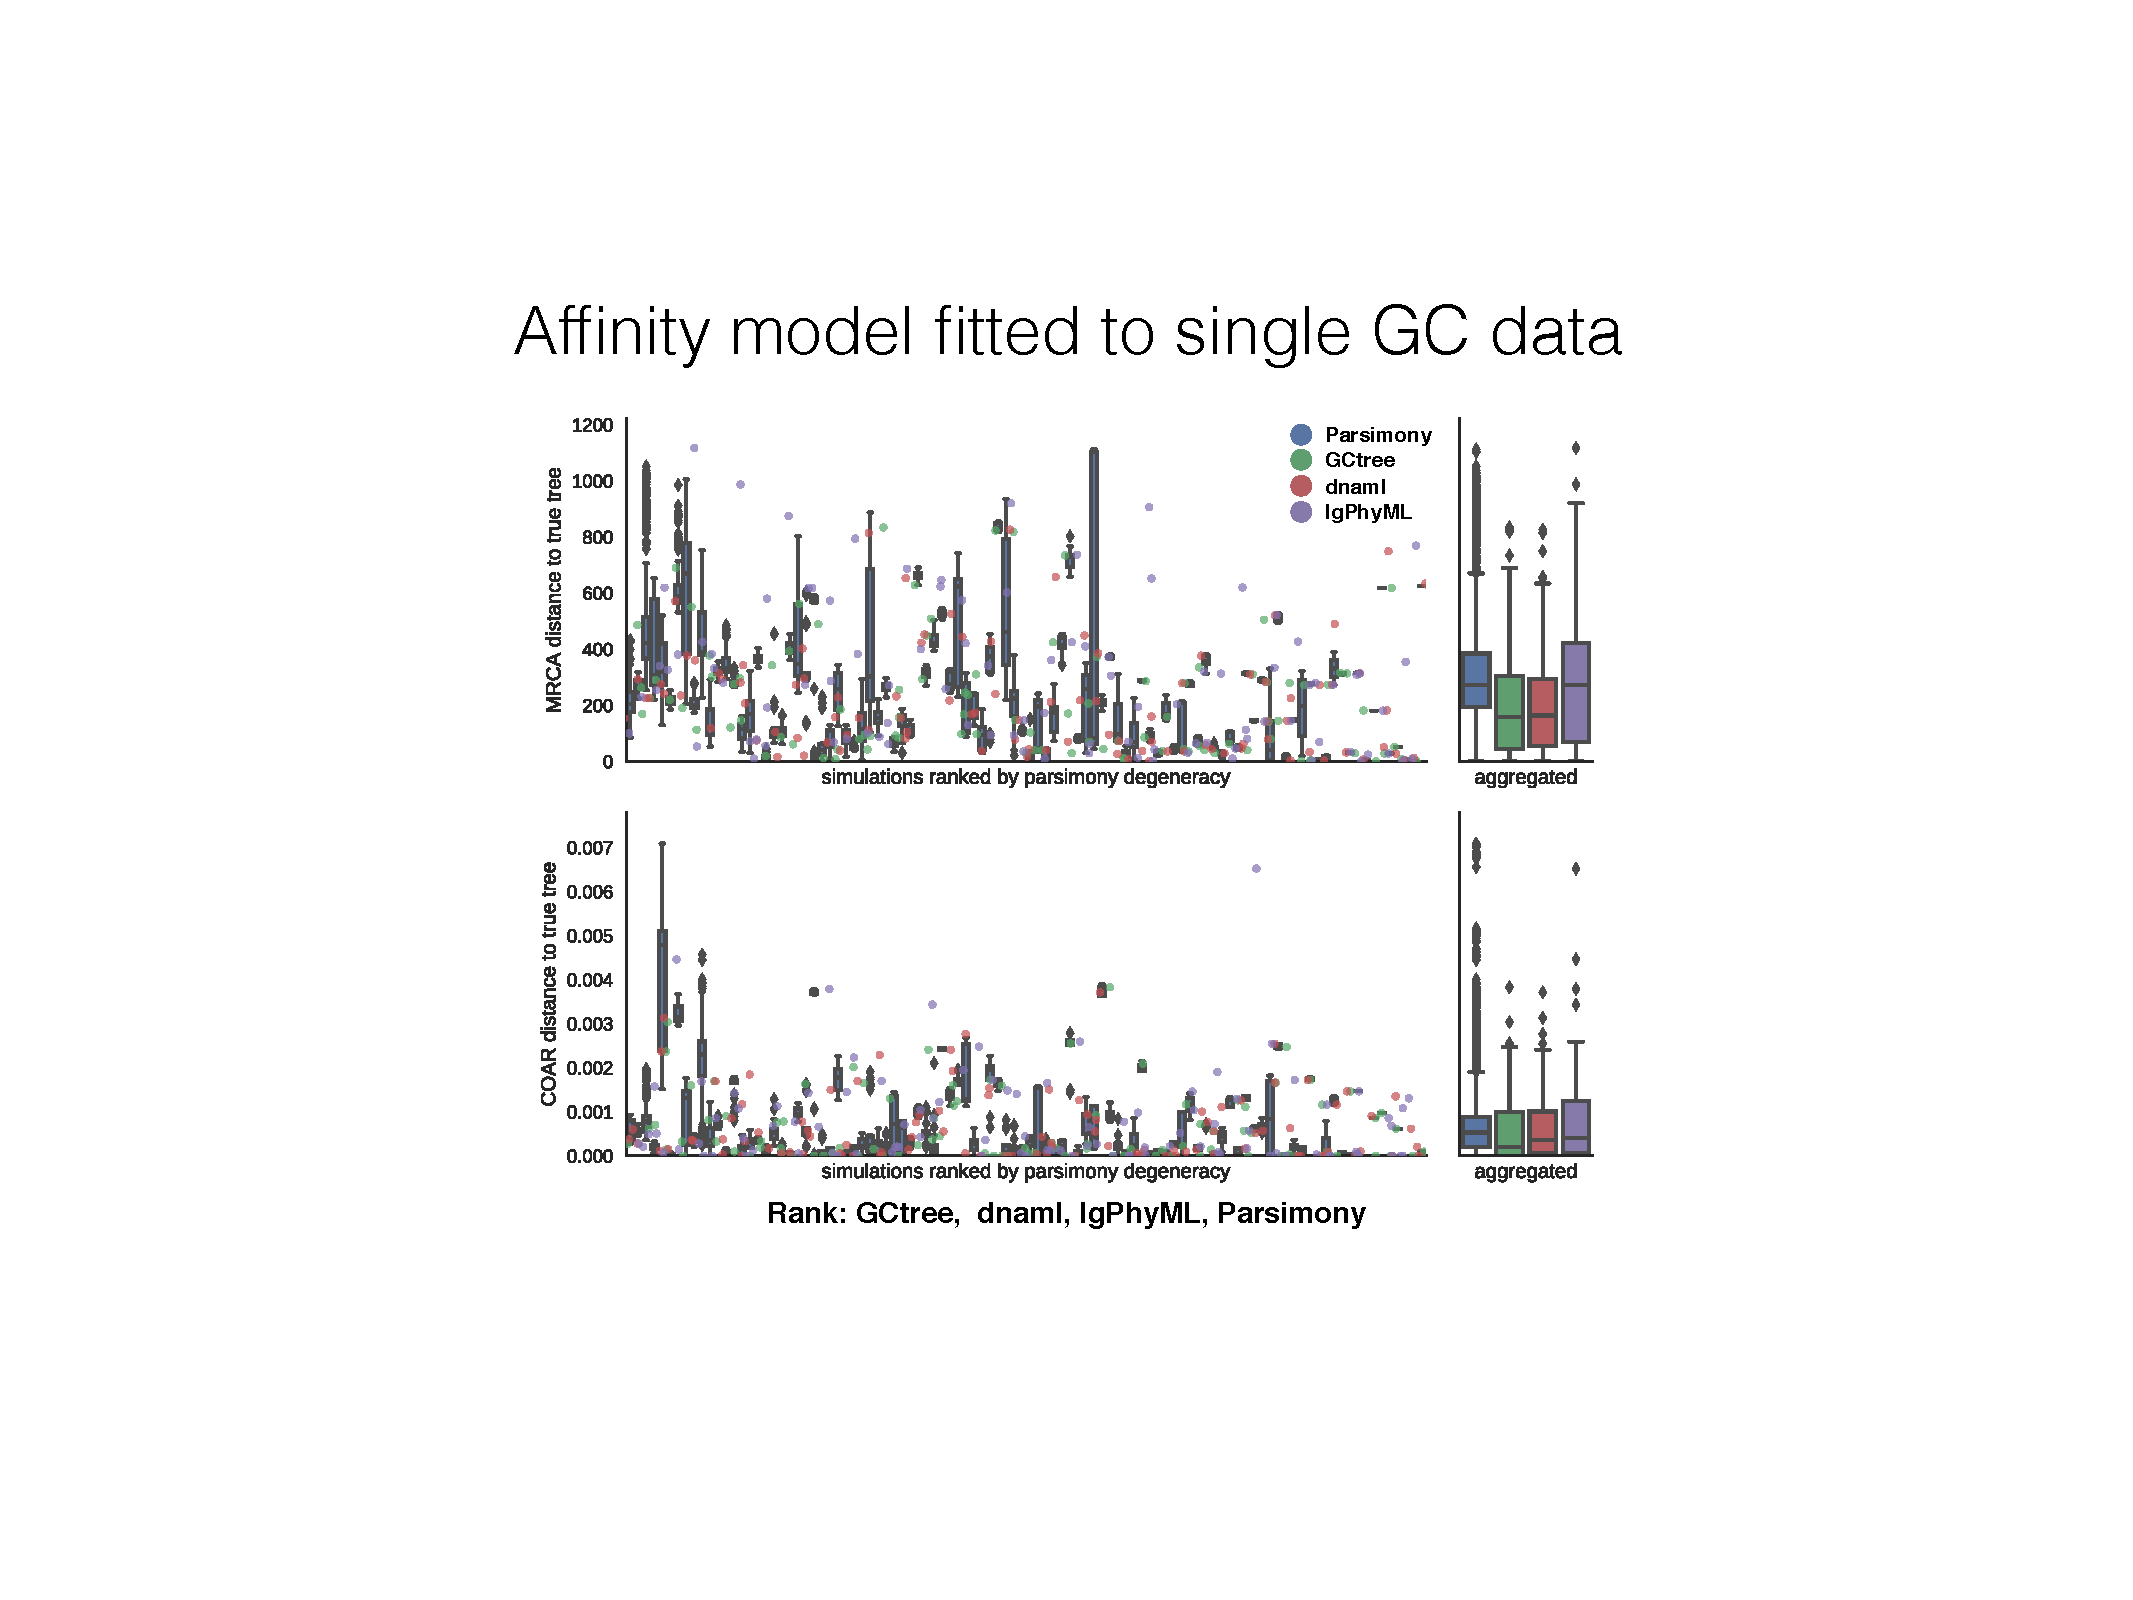
\includegraphics[width=0.8\textwidth]{figures/Tas-affsim_vali.pdf}
    \caption{
        \label{fig:Tas-affsim_vali}
        Performance of different inference method over the 100 simulations shown in \ref{fig:Tas-affsim_runstat}.
        Standard box plot format with the box covering the two middle quartiles (Q2=25\% to Q3=75\% percentile), whiskers extends these and extra 1.5 times the interquartile range and points outside this are plotted individually.
        The median is indicated by a black line.
        A rank of best to worst, is subjectively decided based on the metrics plotted and with importance of the metrics determined by the rank; COAR, MRCA, RF.
    }
\end{figure}

\begin{figure}[!ht]
    \centering
    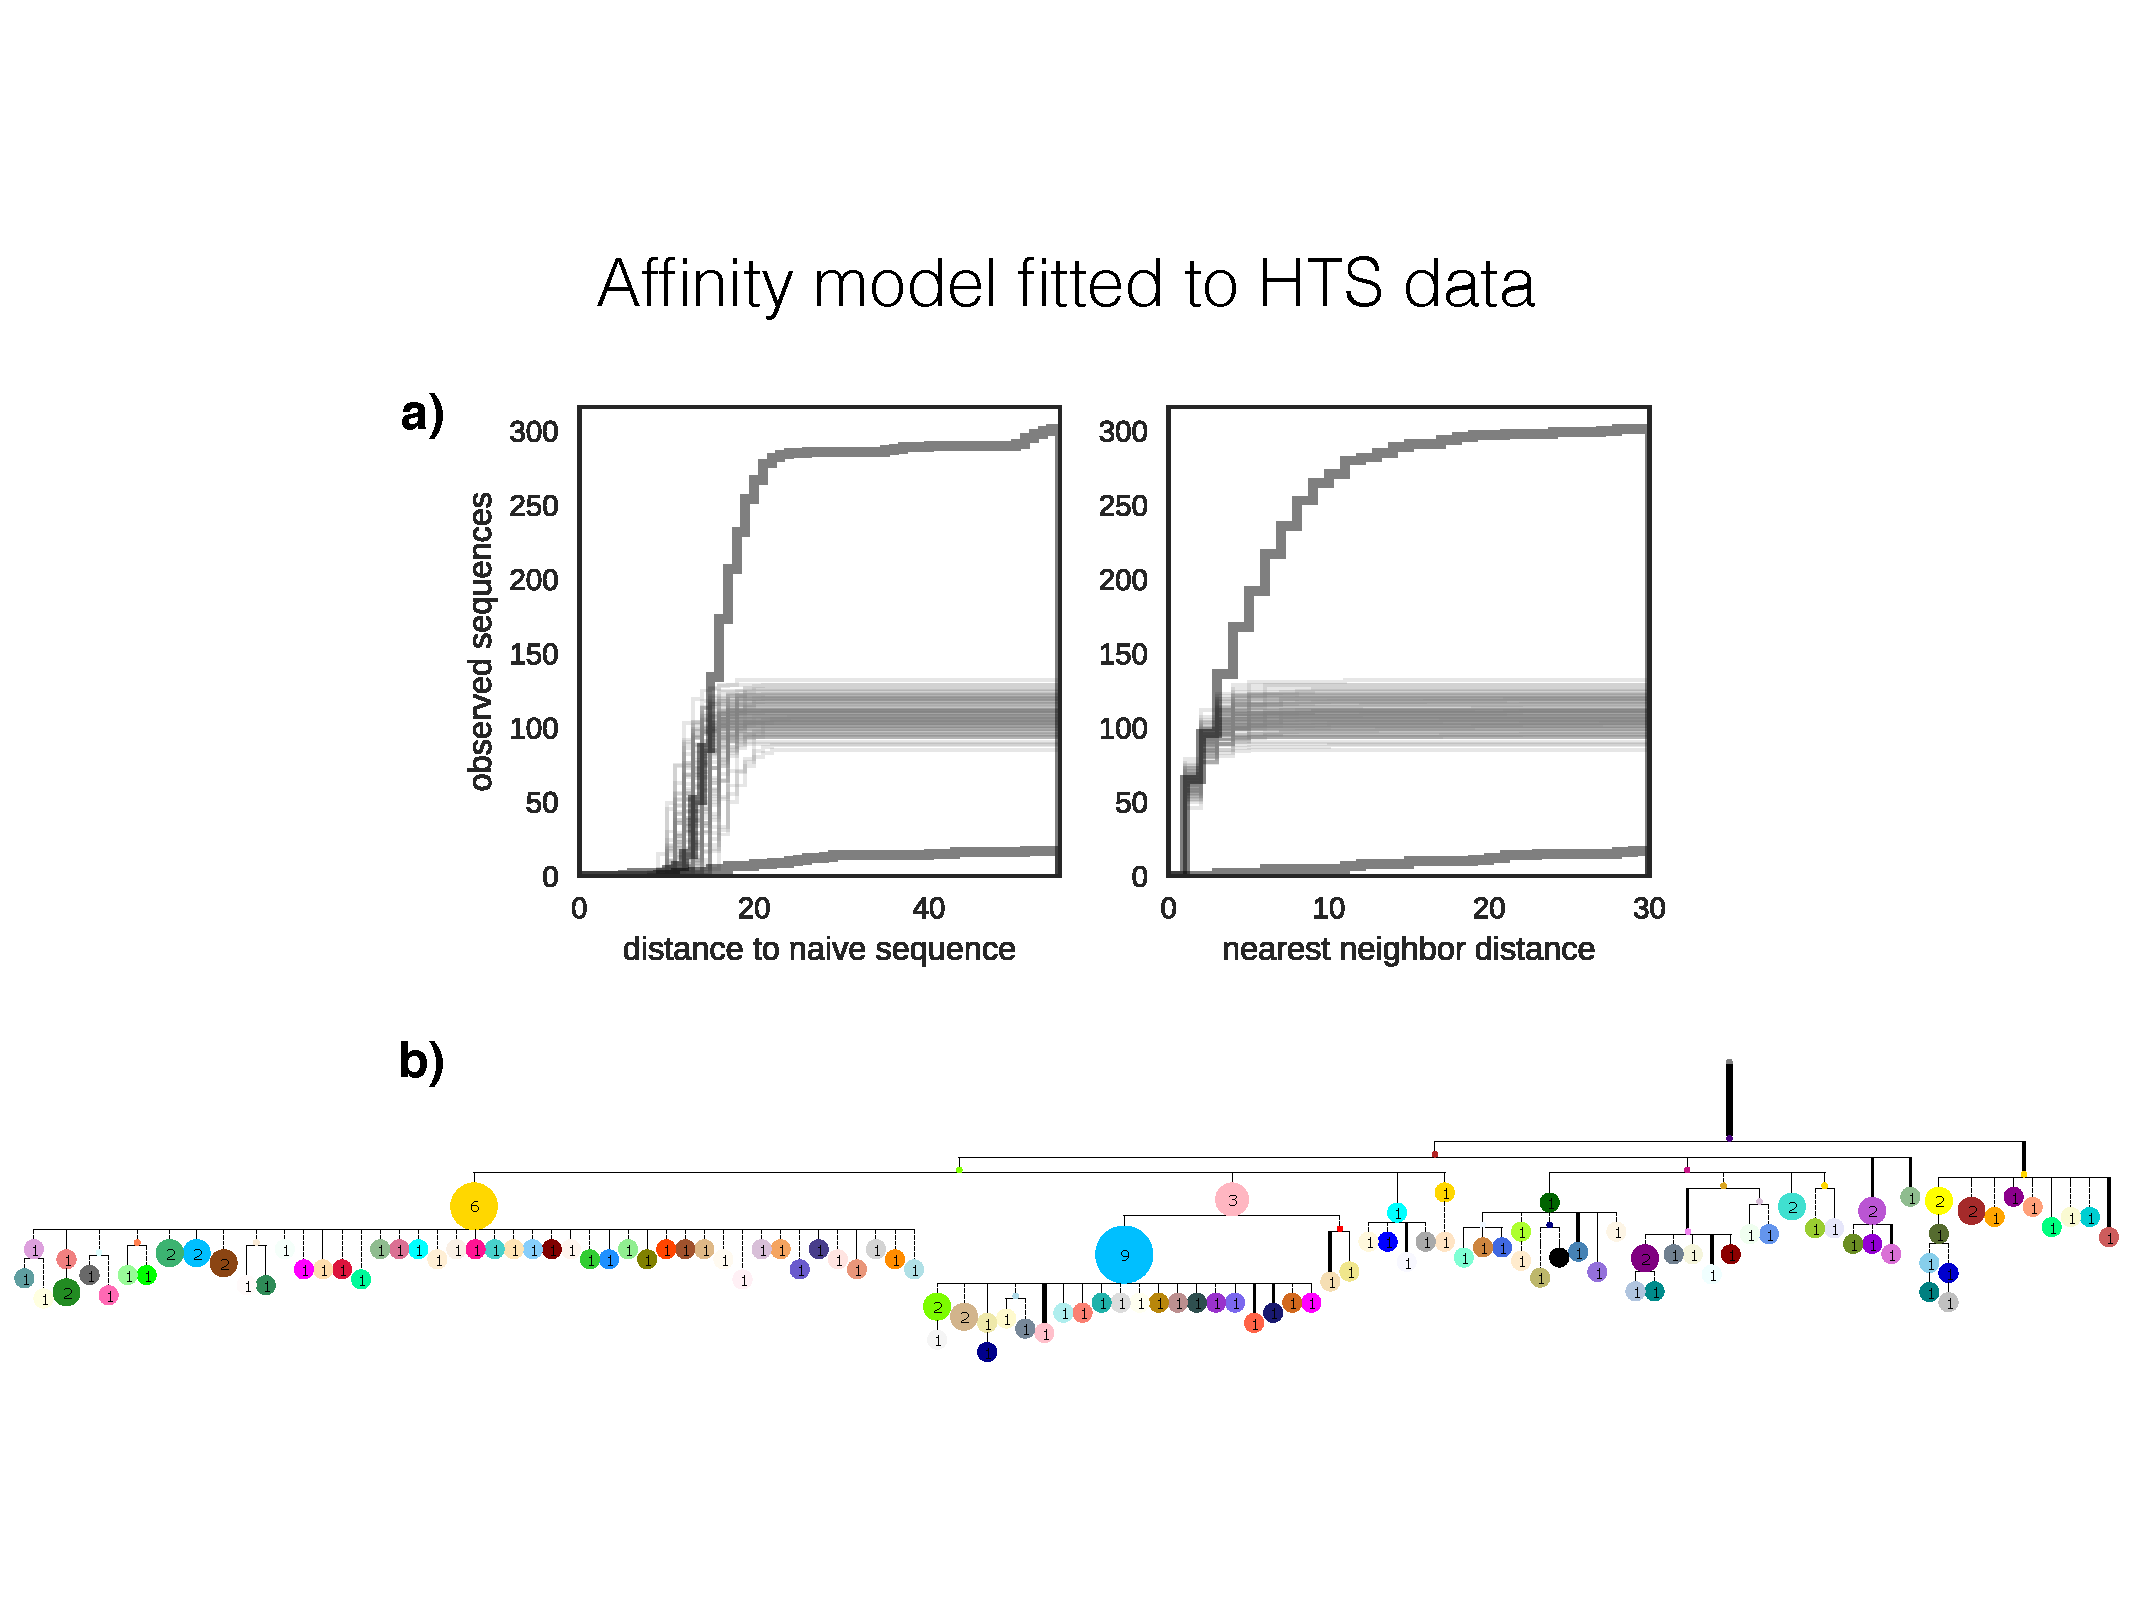
\includegraphics[width=1\textwidth]{figures/Laura-affsim_runstat.pdf}
    \caption{
        \label{fig:Laura-affsim_runstat}
        Affinity simulation with parameters fit to HTS data. In a) summary statistics of how well the simulations fit data (simulations in grey shade, data in dark grey). In b) a typical tree topology from the simulation run.
    }
\end{figure}
\begin{figure}[!ht]
    \centering
    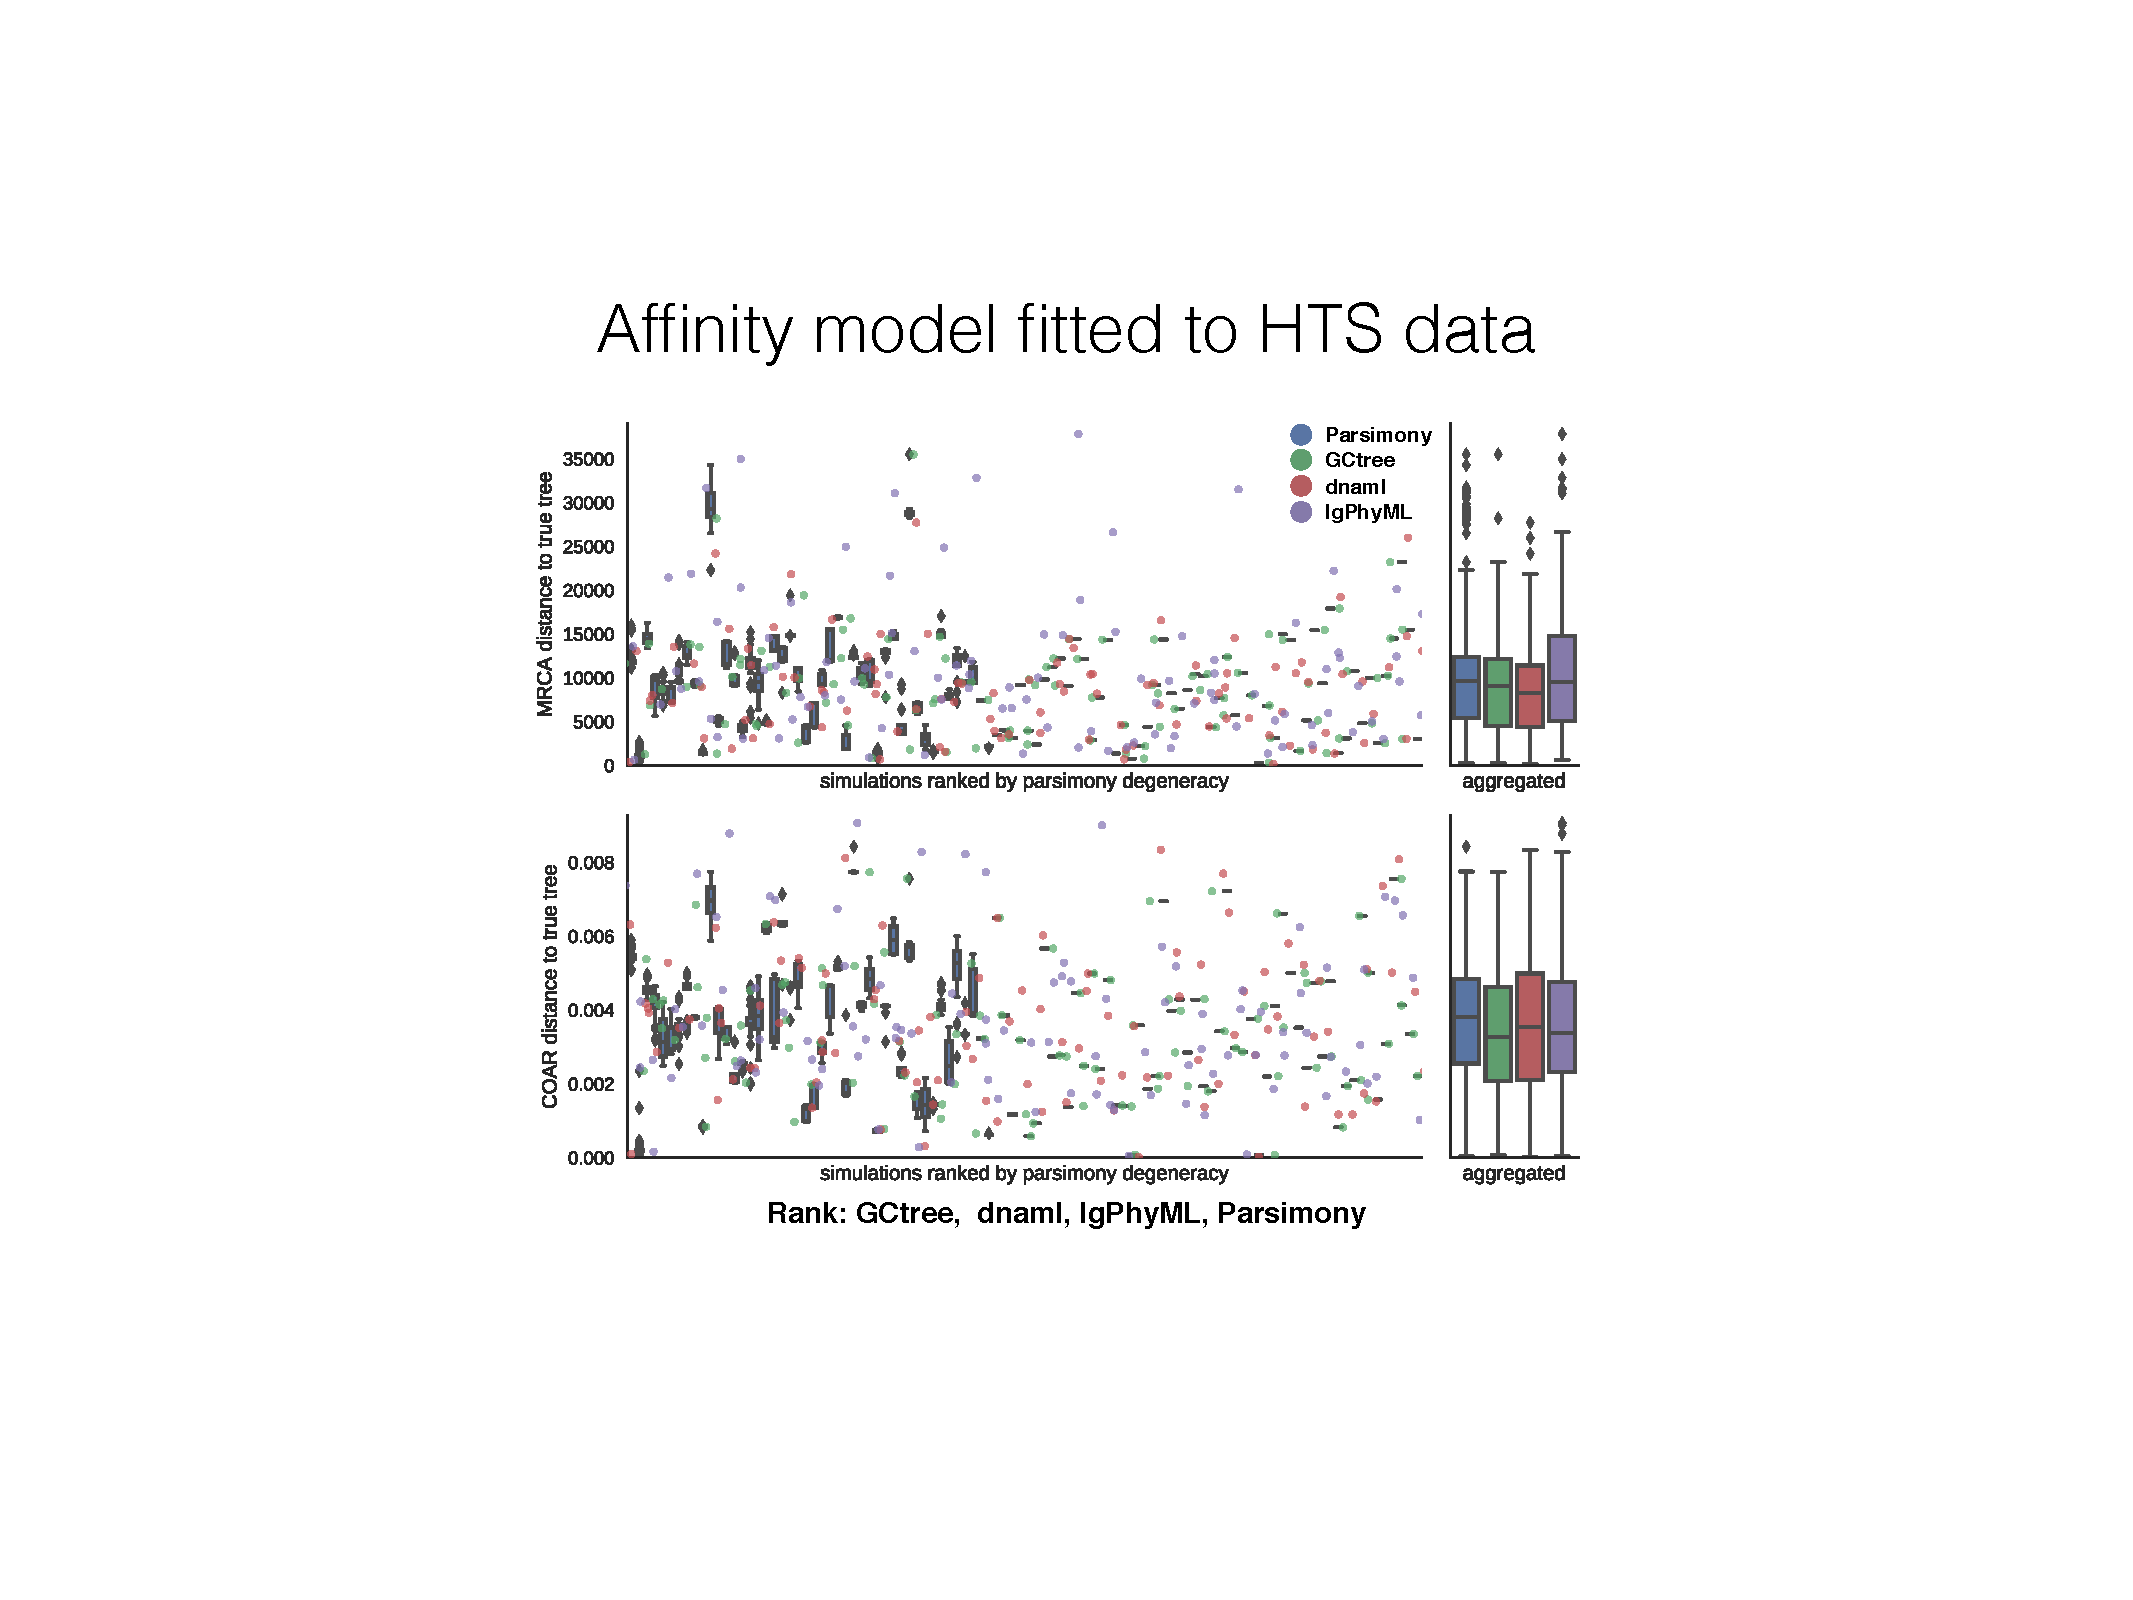
\includegraphics[width=0.8\textwidth]{figures/Laura-affsim_vali.pdf}
    \caption{
        \label{fig:Laura-affsim_vali}
        Performance of different inference method over the 100 simulations shown in \ref{fig:Laura-affsim_runstat}.
        Standard box plot format with the box covering the two middle quartiles (Q2=25\% to Q3=75\% percentile), whiskers extends these and extra 1.5 times the interquartile range and points outside this are plotted individually.
        The median is indicated by a black line.
        A rank of best to worst, is subjectively decided based on the metrics plotted and with importance of the metrics determined by the rank; COAR, MRCA.
    }
\end{figure}







%\fi